\chapter{Analisis}
\label{chap:analisis}
\section{Analisis Sistem Kini}
Seperti dibahas pada bab \ref{sec:judge}, \textit{SharIF Judge} merupakan sebuah \textit{online judge} yang di kustomisasi sesuai dengan kebutuhan Informatika UNPAR. \textit{SharIF Judge} dibentuk menggunakan \textit{framework CodeIgniter 3} yang menerapkan  arsitektur \textit{Model-View-Controller} atau MVC. Arsitektur ini memisahkan pemrosesan data pada \textit{Model}, memisahkan logika pada \textit{Controller}, dan memisahkan tampilan pada \textit{View}. Selain itu terdapat direktori \texttt{assets} yang berisikan seluruh kebutuhan pengguna untuk ditampilkan seperti \textit{javascript} dan gambar.

\subsection{\textit{Model}}
\textit{Model} terdapat pada direktori \texttt{application/models}. Direktori ini berisikan kelas \textit{model} dengan fungsi-fungsi untuk mengolah data pada aplikasi. Berikut merupakan \textit{model} pada \textit{SharIF Judge} beserta fungsi-fungsinya.
\subsubsection{\texttt{Assignment\_model.php}}
\textit{Model Assignment} terdapat beberapa fungsi untuk memproses data pada tabel \textit{assignment}. Berikut merupakan fungsi-fungsi dari \textit{model} tersebut:
\begin{itemize}
	\item \texttt{add\_assignment}\\
	Fungsi ini berguna untuk menambahkan atau memperbaharui \textit{assignment} pada \textit{database}.
	\item \texttt{delete\_assignment}\\
	Fungsi ini berguna untuk menghapus \textit{assignment} pada \textit{database}.
	\item \texttt{all\_assignments}\\
	Fungsi ini berguna untuk mengembalikan seluruh \textit{assignment} beserta informasi \textit{assignment} tersebut.
	\item \texttt{new\_assignment\_id}\\
	Fungsi ini berguna untuk mencari \texttt{id} terkecil yang dapat digunakan untuk menambahkan \textit{assignment} baru.
	\item \texttt{all\_problems}\\
	Fungsi ini berguna untuk mengembalikan seluruh \textit{problems} dari \textit{assignment} yang ada.
	\item \texttt{problem\_info}\\
	Fungsi ini berguna untuk mengembalikan baris tabel untuk \textit{problem} tertentu.
	\item \textit{assignment\_info}\\
	Fungsi ini berguna untuk mengembalikan baris tabel untuk \texttt{assignment} tertentu.
	\item \texttt{is\_participant}\\
	Fungsi ini berguna untuk mengecek apakah \textit{username} merupakan peserta atau tidak.
	\item \texttt{increase\_total\_submits}\\
	Fungsi ini berguna untuk menambahkan satu buah total \textit{submit}.
	\item \texttt{set\_moss\_time}\\
	Fungsi ini berguna untuk memperbaharui \textit{"Moss Update Time"} untuk \textit{assignment} tertentu.
	\item \texttt{get\_moss\_time}\\
	Fungsi ini berguna untuk mengembalikan \textit{"Moss Update Time"} untuk \textit{assignment} tertentu.
	\item \texttt{save\_problem\_description}\\
	Fungsi ini berguna untuk menyimpan atau memperbaharui deskripsi \textit{problem}.
	\item \texttt{\_update\_coefficients}\\
	Fungsi ini dipanggil pada fungsi \texttt{add\_assignment} yang berguna untuk memperbaharui koefisien dari \textit{assignment} tertentu.
\end{itemize}
\subsubsection{\texttt{Hof\_model.php}}
Berikut merupakan fungsi-fungsi dari \texttt{Hof\_model.php} yang berguna untuk mengambil data untuk ditampilkan pada halaman \textit{Hall of Fame}.
\begin{itemize}
	\item \texttt{get\_all\_final\_submission}\\
	Fungsi ini berguna untuk mengambil data untuk \textit{Hall of Fame} berdasarkan \textit{username}.
	\item \texttt{get\_all\_user\_assignments}\\
	Fungsi ini berguna untuk mengambil detail \textit{assignment} dan \textit{problem} berdasarkan pengguna.
\end{itemize}
\subsubsection{\texttt{Logs\_model.php}}
Berikut merupakan fungsi-fungsi dari \texttt{Logs\_model.php} yang berguna untuk mencatat \textit{log} pada beberapa tabel.
\begin{itemize}
	\item \texttt{insert\_to\_logs}\\
	Fungsi ini berguna untuk mencatat \textit{log} pada tabel \textit{login}.
	\item \texttt{get\_all\_logs}\\
	Fungsi ini berguna untuk mengembalikan seluruh \textit{log} dalam bentuk \textit{array}.
\end{itemize}
\subsubsection{\texttt{Notifications\_model.php}}
\textit{Notifications Assignment} terdapat beberapa fungsi untuk memproses data pada tabel \textit{notifications}. Berikut merupakan fungsi-fungsi dari \textit{model} tersebut:
\begin{itemize}
	\item \texttt{get\_all\_notifications}\\
	Fungsi ini berguna untuk mengembalikan seluruh \textit{notifications} dalam bentuk \textit{array}.
	\item \texttt{get\_latest\_notifications}\\
	Fungsi ini berguna untuk mengembalikan sepuluh \textit{notification} terakhir.
	\item \texttt{add\_notification}\\
	Fungsi ini berguna untuk menambahkan \textit{notification} baru.
	\item \texttt{update\_notification}\\
	Fungsi ini berguna untuk memperbaharui \textit{notification} tertentu.
	\item \texttt{delete\_notification}\\
	Fungsi ini berguna untuk menghapus \textit{notification} tertentu.
	\item \texttt{get\_notification}\\
	Fungsi ini berguna untuk mengembalikan \textit{notification} dalam bentuk \textit{array}.
	\item \texttt{have\_new\_notification}\\
	Fungsi ini berguna untuk mengecek apakah terdapat \textit{notification} setelah waktu tertentu.
\end{itemize}
\subsubsection{\texttt{Queue\_model.php}}
Berikut merupakan fungsi-fungsi dari \texttt{Queue\_model.php} yang berguna untuk memproses data pada halaman \textit{queue}.
\begin{itemize}
	\item \texttt{in\_queue}\\
	Fungsi ini berguna untuk mengecek apakah \textit{submission} pengguna tertentu sudah dalam antrean.
	\item \texttt{get\_queue}\\
	Fungsi ini berguna untuk mengembalikan data seluruh antrian.
	\item \texttt{empty\_queue}\\
	Fungsi ini berguna untuk menghapus seluruh tabel \textit{queue}.
	\item \texttt{add\_to\_queue}\\
	Fungsi ini berguna untuk memasukan \textit{submission} kedalam tabel \textit{queue}.
	\item \texttt{rejudge}\\
	Fungsi ini berguna untuk menambahkan \textit{submission} kedalam antrean untuk dilakukan \textit{rejudge}.
	\item \texttt{rejudge\_single}\\
	Fungsi ini berguna untuk menambahkan satu buah \textit{submission} kedalam antrean untuk dilakukan \textit{rejudge}.
	\item \texttt{get\_first\_item}\\
	Fungsi ini berguna untuk mengambil data pertama dalam antrean.
	\item \texttt{remove\_item}\\
	Fungsi ini berguna untuk menghapus data tertentu dalam antrean.
	\item \texttt{save\_judge\_result\_in\_db}\\
	Fungsi ini berguna untuk menyimpan hasil dari \textit{judge} ke dalam \textit{database}.
	\item \texttt{add\_to\_queue\_exec}\\
	Fungsi ini berguna untuk menambahkan data \textit{dummy} pada antrean.
\end{itemize}
\subsubsection{\texttt{Scoreboard\_model.php}}
Berikut merupakan fungsi-fungsi dari \texttt{Scoreboard\_model.php} yang berguna untuk memproses data untuk ditampilkan pada halaman \textit{Score Board}.
\begin{itemize}
	\item \texttt{\_generate\_scoreboard}\\
	Fungsi ini dipanggil pada fungsi \texttt{update\_scoreboard} dan berfungsi untuk menghasilkan \textit{scoreboard} dari \textit{final submission}.
	\item \texttt{update\_scoreboards}\\
	Fungsi ini berguna untuk memperbaharui \textit{cache scoreboard} dari seluruh \textit{assignment}. Fungsi ini dipanggil setiap terdapat penghapusan pengguna atau seluruh \textit{assignment} pengguna.
	\item \texttt{update\_scoreboard}\\
	Fungsi ini berguna untuk memperbaharui \textit{cache scoreboard} dari seluruh \textit{assignment}. Fungsi ini dipanggil setelah \textit{judge} atau \textit{rejudge}.
	\item \texttt{get\_scoreboard}\\
	Fungsi ini berguna untuk mengambil seluruh \textit{cache scoreboard} dari \textit{assignment} tertentu.
\end{itemize}
\subsubsection{\texttt{Settings\_model.php}}
Berikut merupakan fungsi-fungsi dari \texttt{Settings\_model.php} yang berguna untuk memproses data untuk ditampilkan pada tabel \textit{settings}.
\begin{itemize}
	\item \texttt{get\_setting}\\
	Fungsi ini berguna untuk mengembalikan data \textit{setting} tertentu.
	\item \texttt{set\_setting}\\
	Fungsi ini berguna untuk memperbaharui \textit{setting}.
	\item \texttt{get\_all\_settings}\\
	Fungsi ini berguna untuk mengembalikan seluruh data \textit{setting}.
	\item \texttt{set\_settings}\\
	Fungsi memperbaharui beberapa \textit{setting}.
\end{itemize}
\subsubsection{\texttt{Submit\_model.php}}
Berikut merupakan fungsi-fungsi dari \texttt{Submit\_model.php} yang berguna untuk memproses data yang berkaitan dengan \textit{submission}.
\begin{itemize}
	\item \texttt{get\_submission}\\
	Fungsi ini berguna untuk mengembalikan baris data \textit{submission} tertentu.
	\item \texttt{get\_final\_submissions}\\
	Fungsi ini berguna untuk mengembalikan seluruh \textit{final submission}.
	\item \texttt{get\_all\_submissions}\\
	Fungsi ini berguna untuk mengembalikan seluruh \textit{submission}.
	\item \texttt{count\_final\_submissions}\\
	Fungsi ini berguna untuk menghitung seluruh \textit{final submission}.
	\item \texttt{count\_all\_submissions}\\
	Fungsi ini berguna untuk menghitung seluruh \textit{submission}.
	\item \texttt{set\_final\_submission}\\
	Fungsi ini berguna untuk memperbaharui \textit{submission} terentu menjadi \textit{final submission}.
	\item \texttt{add\_upload\_only}\\
	Fungsi ini berguna untuk menambahkan hasil dari \textit{upload only} ke dalam \textit{database}.
\end{itemize}
\subsubsection{\textit{User\_model.php}}
Berikut merupakan fungsi-fungsi dari \texttt{User\_model.php} yang berguna untuk memproses data pada tabel \textit{users}.
\begin{itemize}
	\item \texttt{have\_user}\\
	Fungsi ini berguna untuk mengecek apakah terdapat pengguna dengan \textit{username} tertentu.
	\item \texttt{user\_id\_to\_username}\\
	Fungsi ini berguna untuk mengembalikan \textit{user id} menjadi \textit{username}.
	\item \texttt{username\_to\_user\_id}\\
	Fungsi ini berguna untuk mengembalikan \textit{username} menjadi \textit{user id}.
	\item \texttt{have\_email}\\
	Fungsi ini berguna untuk mengecek apakah terdapat \textit{username} dengan \textit{email} tertentu.
	\item \texttt{add\_user}\\
	Fungsi ini berguna untuk menambahkan sebuah pengguna.
	\item \texttt{add\_users}\\
	Fungsi ini berguna untuk menambahkan banyak pengguna.
	\item \texttt{delete\_user}\\
	Fungsi ini berguna untuk menghapus pengguna tertentu.
	\item \texttt{delete\_submissions}\\
	Fungsi ini berguna untuk menghapus seluruh \textit{submission} pada pengguna tertentu.
	\item \texttt{validate\_user}\\
	Fungsi ini berguna untuk mengecek \textit{username} dan \textit{password} apakah sesuai dengan data.
	\item \texttt{selected\_assignment}\\
	Fungsi ini berguna untuk mengembalikan \textit{assignment} untuk pengguna tertentu.
	\item \texttt{get\_names}\\
	Fungsi ini berguna untuk mengembalikan nama dari pengguna tertentu.
	\item \texttt{update\_profile}\\
	Fungsi ini berguna untuk memperbaharui profil dari pengguna seperti nama, \textit{email, password}, dan \textit{role}.
	\item \texttt{send\_password\_reset\_mail}\\
	Fungsi ini berguna untuk menghasilkan \textit{password reset key} dan mengirim \textit{email} untuk melakukan \textit{reset password}.
	\item \texttt{passchange\_is\_valid}\\
	Fungsi ini berguna untuk mengecek apakah \textit{password key} yang diberikan sesuai atau tidak.
	\item \texttt{reset\_password}\\
	Fungsi ini berguna untuk mengatur ulang \textit{password} sesuai dengan \textit{password key} tertentu.
	\item \texttt{get\_all\_users}\\
	Fungsi ini berguna untuk mengembalikan seluruh pengguna untuk halaman \textit{users}.
	\item \texttt{get\_user}\\
	Fungsi ini berguna untuk mengembalikan baris data untuk pengguna tertentu.
	\item \texttt{update\_login\_time}\\
	Fungsi ini berguna untuk memperbaharui \textit{login time} dan \textit{last login time} untuk pengguna tertentu.
\end{itemize}
\subsubsection{\textit{User.php}}
Berikut merupakan fungsi-fungsi dari \texttt{User.php} yang berguna untuk memproses data pada tabel \textit{users}.
\begin{itemize}
	\item \texttt{select\_assignment}\\
	Fungsi ini berguna untuk mengatur \textit{assignment} yang dipilih oleh pengguna.
	\item \texttt{save\_widget\_positions}\\
	Fungsi ini berguna untuk memperbaharui posisi dari \textit{dashboard widget} pada \textit{database}.
	\item \texttt{get\_widget\_positions}\\
	Fungsi ini berguna untuk mengembalikan data \textit{dashboard widget}.
\end{itemize}

%\subsection{\textit{View}}
%\subsubsection{Halaman pada \textit{SharIF Judge}}
%Halaman pada \textit{SharIF Judge} dibagi berdasarkan \textit{role} penggunanya. Setiap role memiliki tampilan halaman berbeda dengan fitur-fitur berbeda setiap \textit{role} penggunanya. Berikut merupakan halaman dan fitur pada \textit{SharIF Judge}:

\subsection{\textit{View}}
\textit{View} terdapat pada direktori \texttt{application/views}. Direktori ini berisikan seluruh \textit{file} untuk tampilan halaman \textit{SharIF Judge}. \textit{File} tersebut dipisahkan oleh direktori sesuai dengan fungsinya. Direktori tersebut dibagi menjadi tiga buah direktori utama yakni \textit{error, pages}, dan \textit{templates}. Direktori \textit{error} berisikan tampilan halaman \textit{error} yang akan dilihat oleh pengguna. Direktori \textit{pages} merupakan tampilan utama \textit{SharIF Judge} yang terbagi lagi menjadi dua buah direktori yakni \textit{admin} dan \textit{authentication}. Direktori \textit{admin} berisikan tampilan halaman untuk \textit{role admin}. Direktori \textit{authentication} berisikan tampilan halaman untuk akses pengguna seperti \textit{LOgin, Register,} dan \textit{Reset Password}. Direktori \textit{templates} terdiri dari tampilan yang digunakan oleh seluruh tampilan halaman seperti \textit{header} dan \textit{side bar}. Berikut merupakan tampilan halaman pada \textit{SharIF Judge}:

\subsubsection{\textit{Dashboard}}
\begin{figure}[H]
	\centering  
	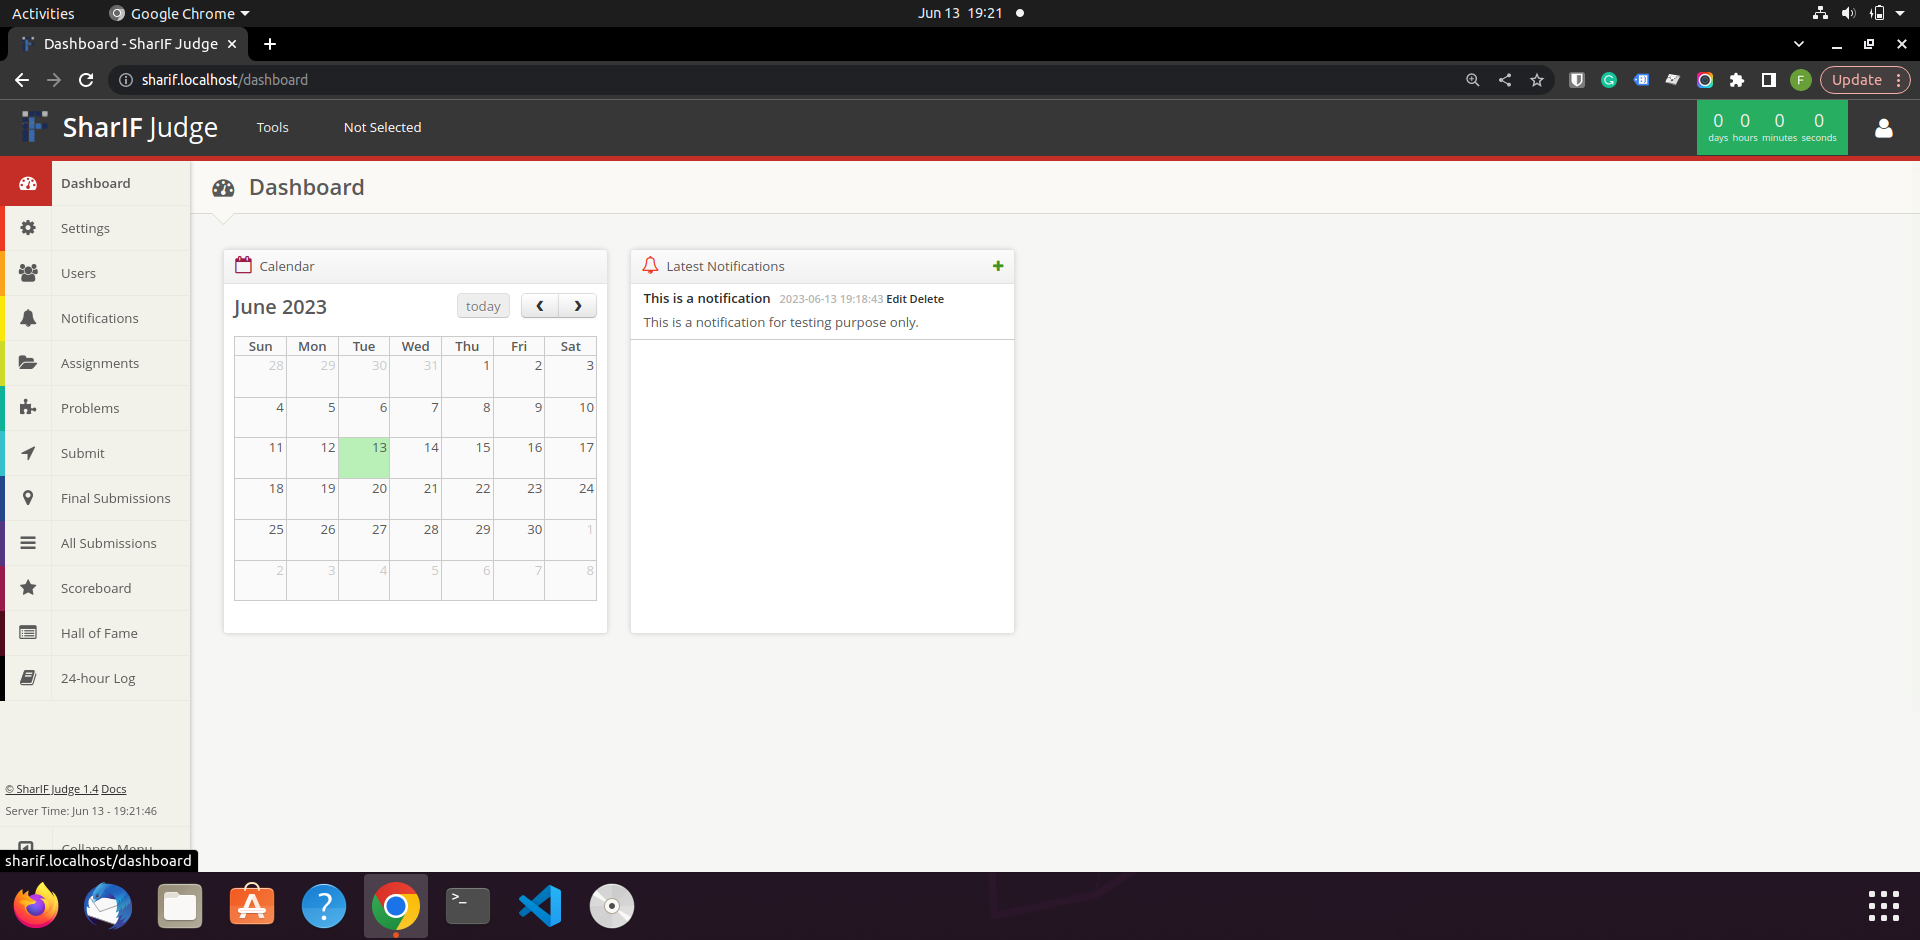
\includegraphics[scale=0.4]{dashboard}  
	\caption[Tampilan Halaman \textit{Dashboard}]{Tampilan Halaman Dashboard} 
	\label{fig:dashboard} 
\end{figure} 

Gambar \ref{fig:dashboard} merupakan tampilan halaman \textit{dashboard} yang terdapat pada semua \textit{role} pengguna.
\subsubsection{\textit{Profile}}
\begin{figure}[H]
	\centering  
	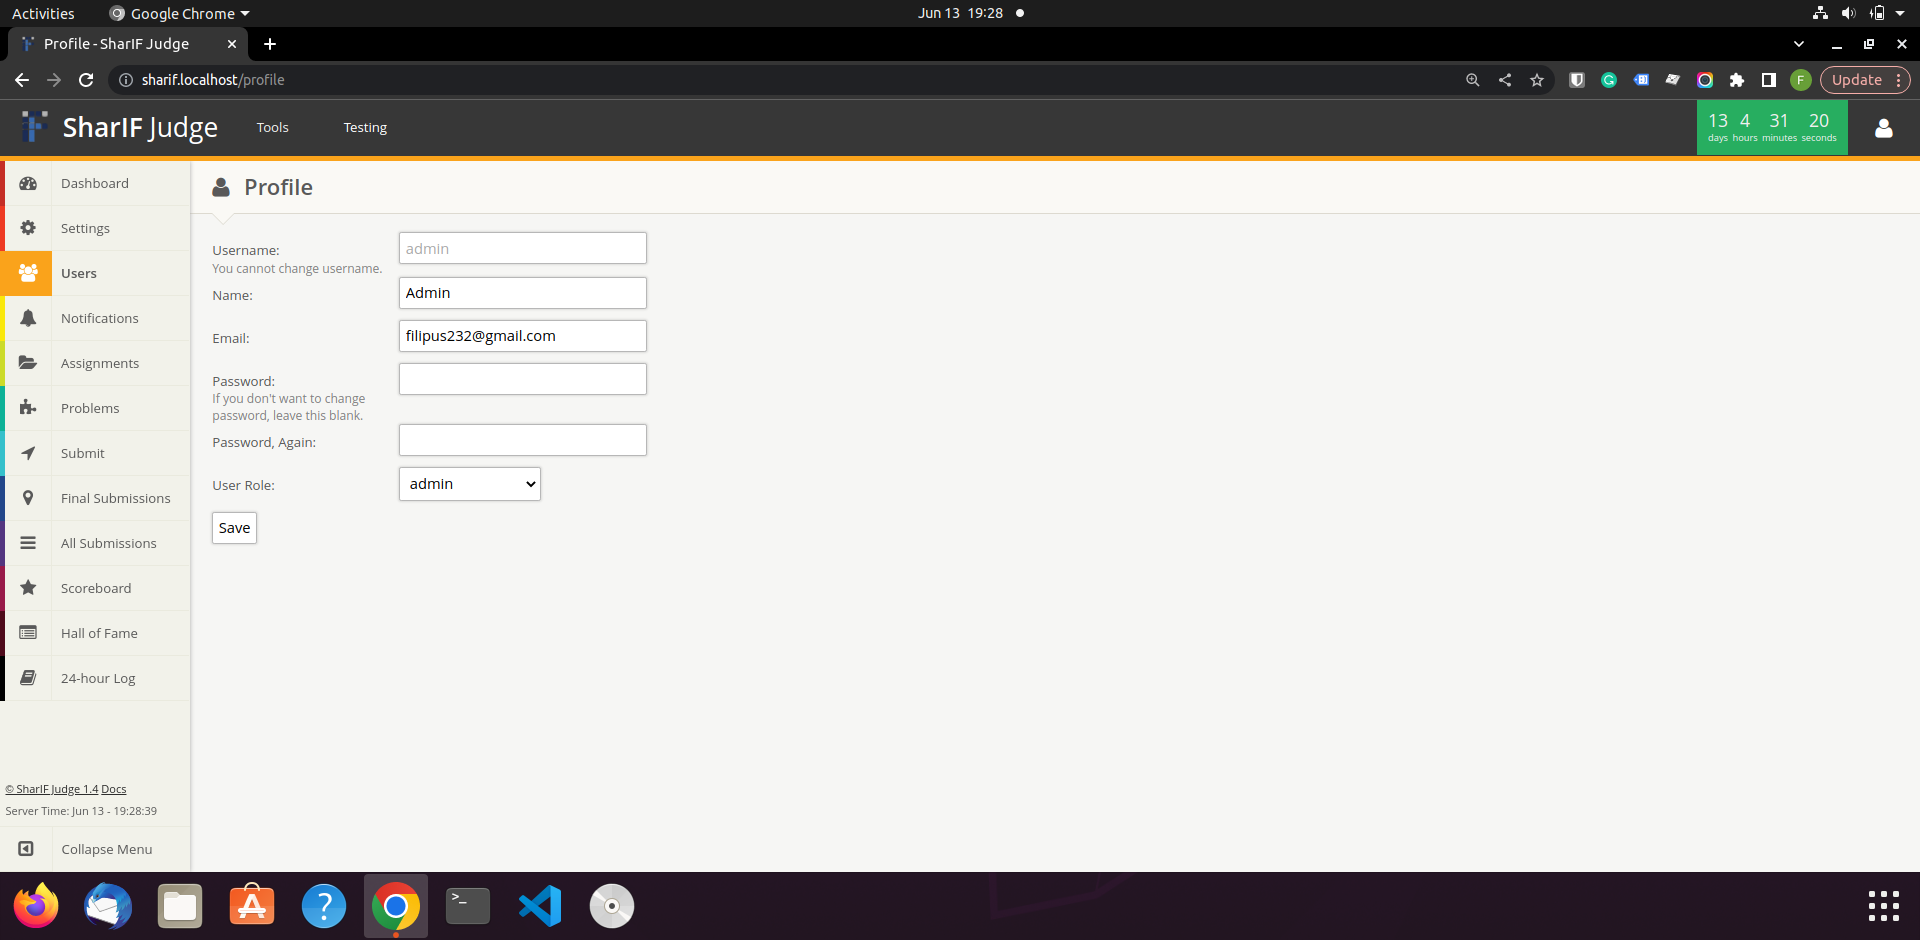
\includegraphics[scale=0.4]{profile}  
	\caption[Tampilan Halaman \textit{Profile}]{Tampilan Halaman Profile} 
	\label{fig:profile} 
\end{figure}

Gambar \ref{fig:profile} merupakan tampilan halaman \textit{profile} yang terdapat pada semua \textit{role} pengguna. Namun, terdapat fitur yang tidak dapat digunakan oleh \textit{siswa} dan \textit{instructor} yakni mengganti role.

\subsubsection{\textit{Settings}}
\begin{figure}[H]
	\centering  
	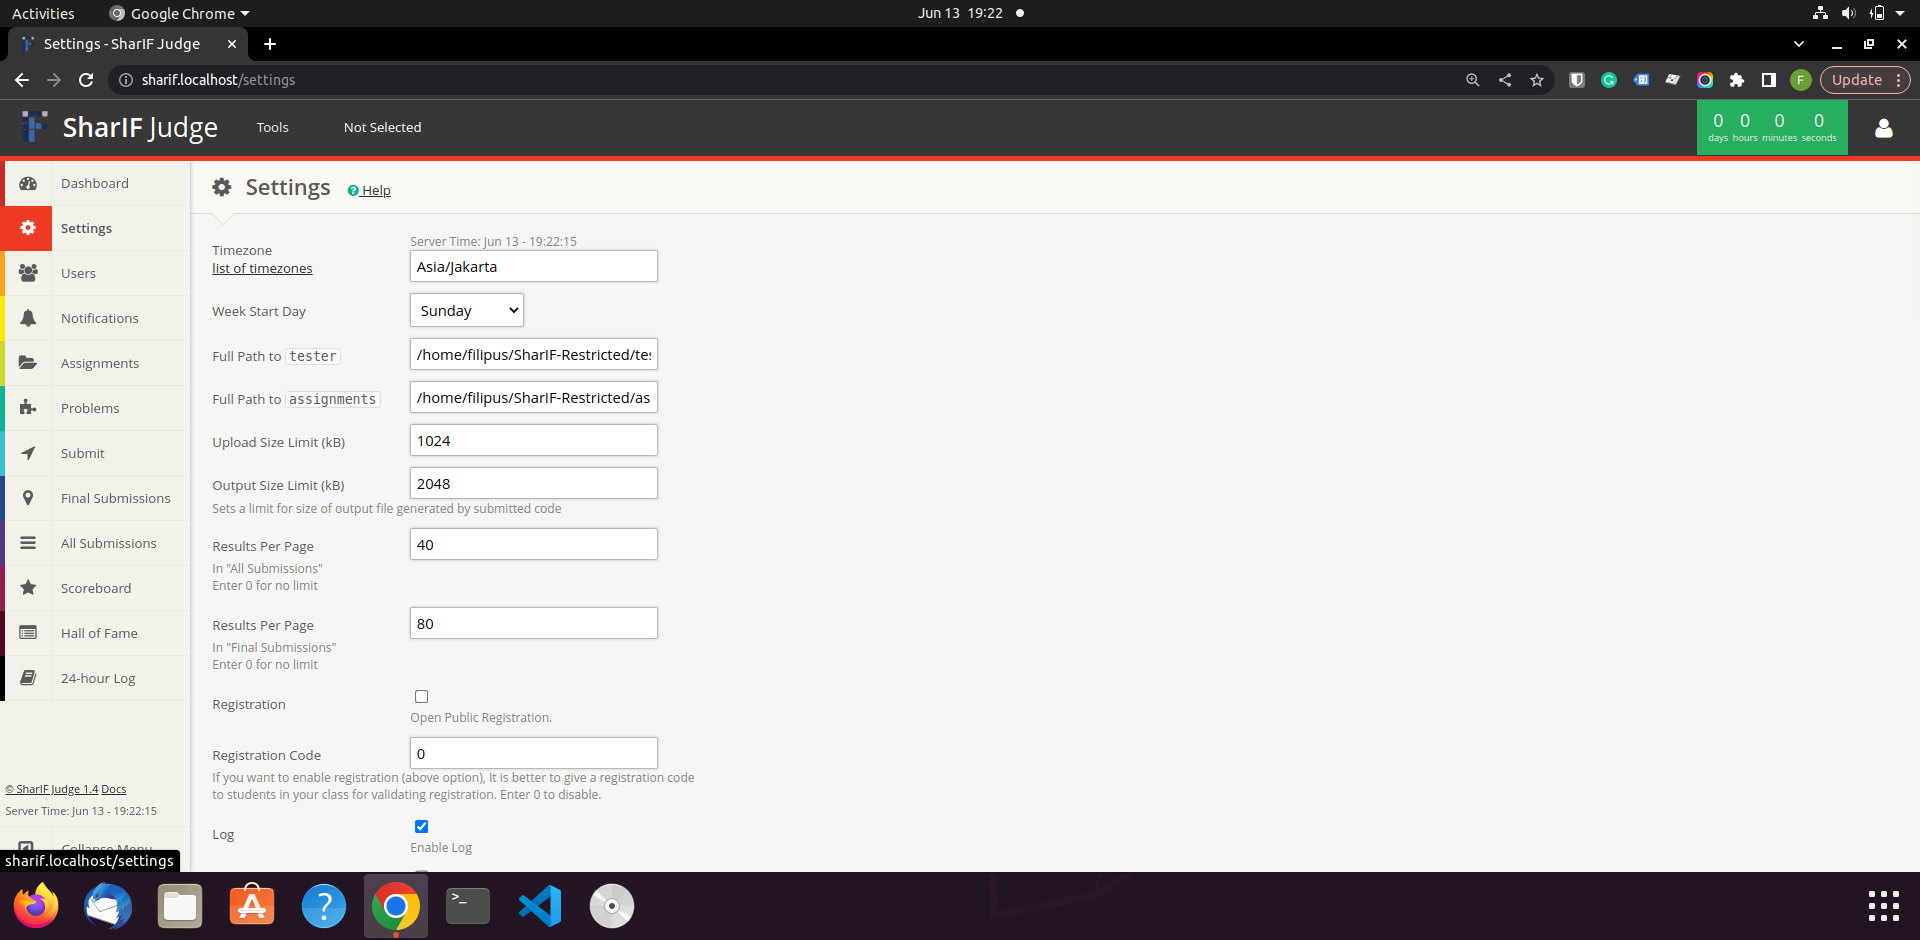
\includegraphics[scale=0.4]{settings}  
	\caption[Tampilan Halaman \textit{Settings}]{Tampilan Halaman Settings} 
	\label{fig:settings} 
\end{figure}

Gambar \ref{fig:settings} merupakan tampilan halaman \textit{settings} yang terdapat hanya pada \textit{role} admin dan \textit{head instructor}. 

\subsubsection{\textit{Users}}
\begin{figure}[H]
	\centering  
	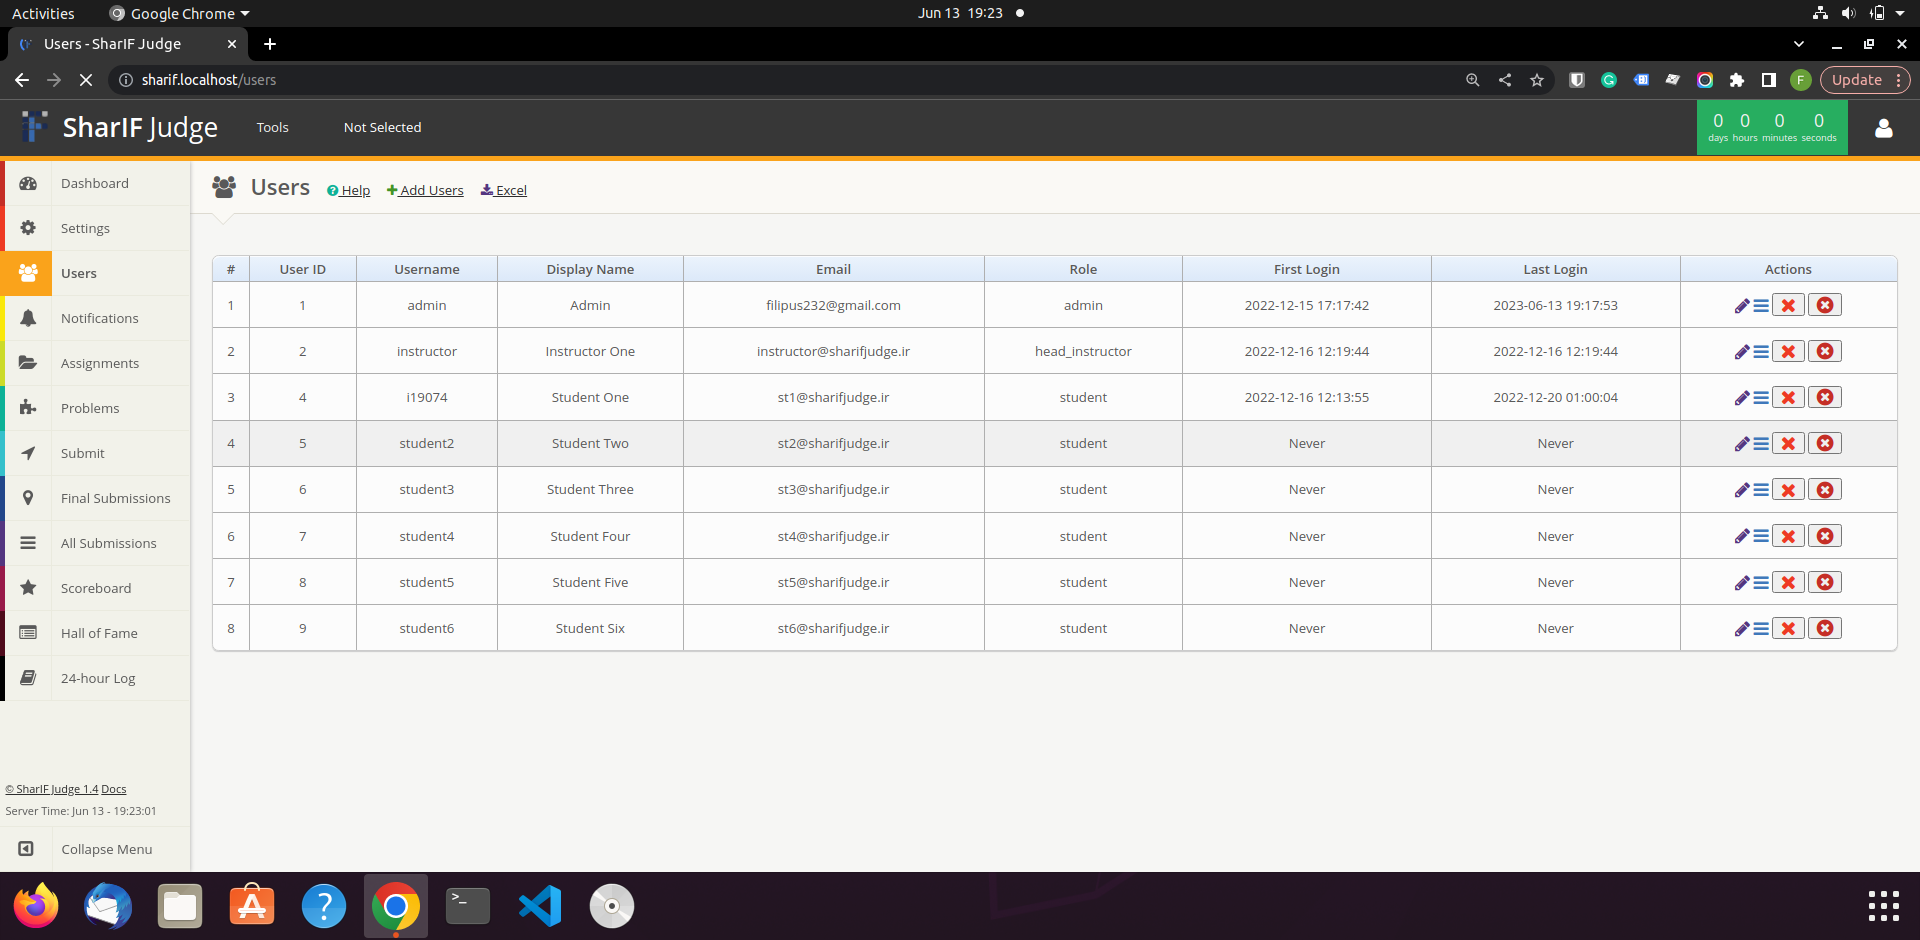
\includegraphics[scale=0.4]{users}  
	\caption[Tampilan Halaman \textit{Users}]{Tampilan Halaman Users} 
	\label{fig:users} 
\end{figure}

Gambar \ref{fig:users} merupakan tampilan halaman \textit{users} yang terdapat hanya pada \textit{role} admin dan \textit{head instructor}.

\subsubsection{\textit{Notifications}}
\begin{figure}[H]
	\centering  
	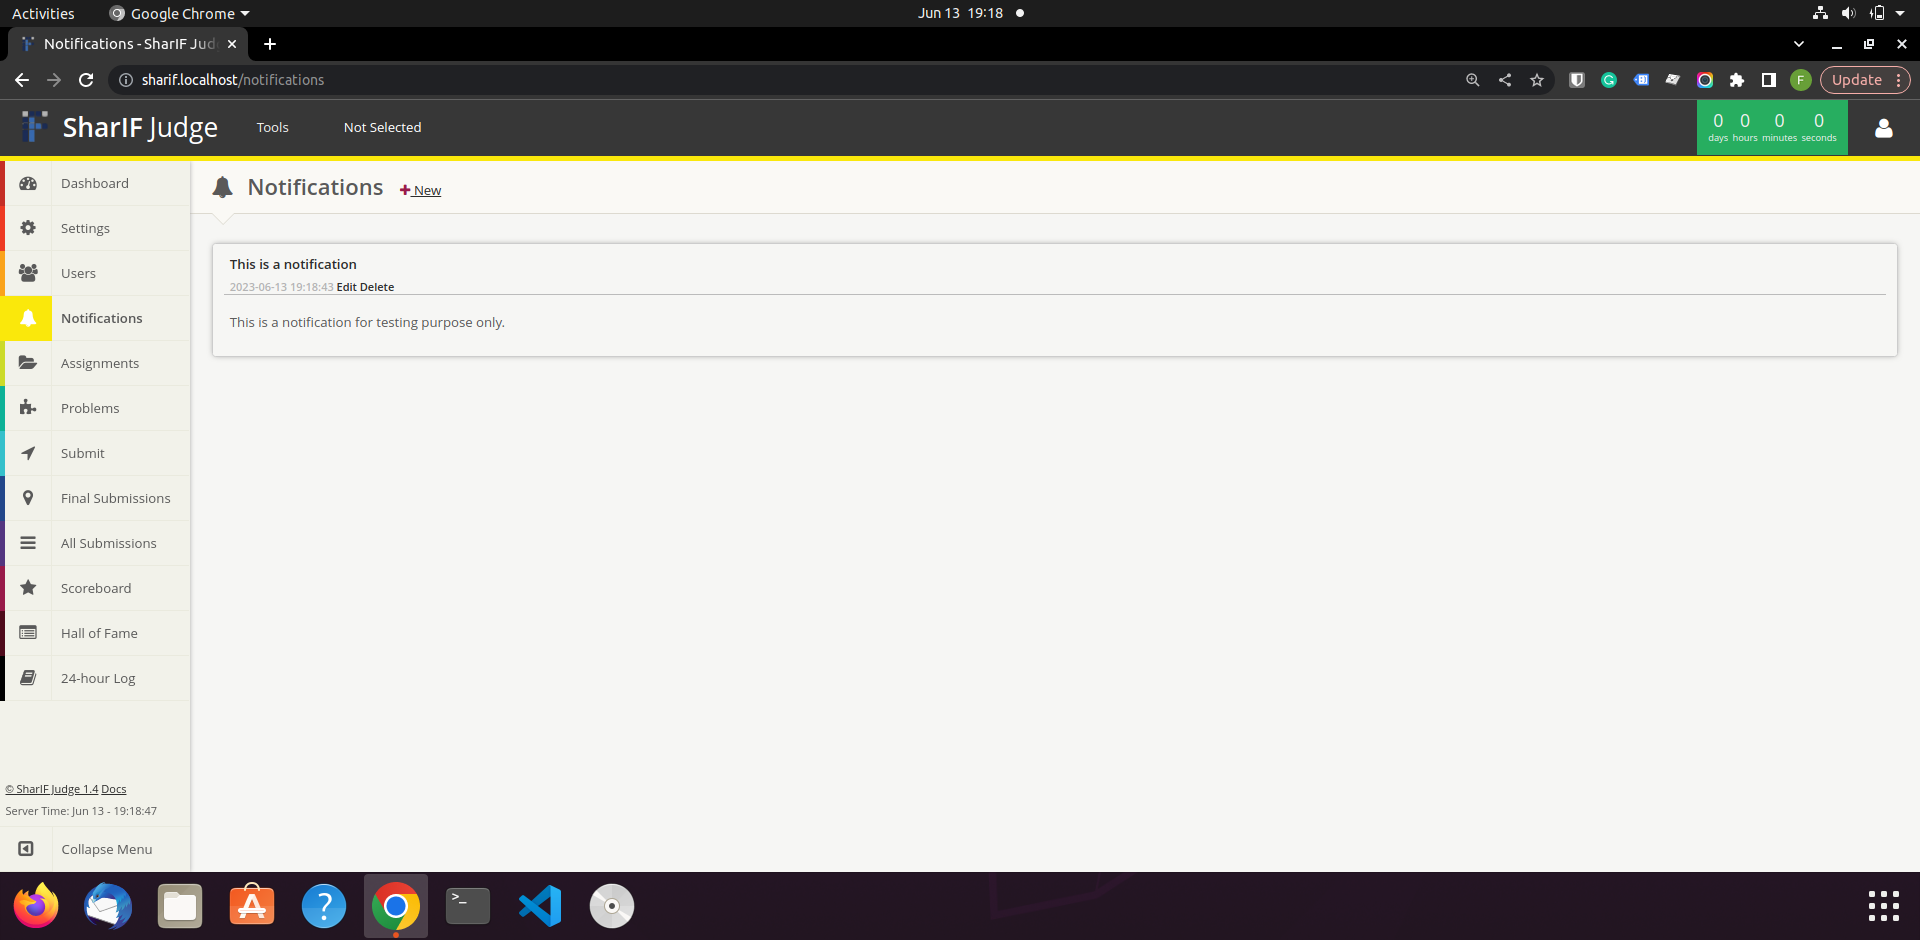
\includegraphics[scale=0.4]{notifications}  
	\caption[Tampilan Halaman \textit{Notifications}]{Tampilan Halaman Notifications} 
	\label{fig:notifications} 
\end{figure}

Gambar \ref{fig:notifications} merupakan tampilan halaman \textit{notifications} yang terdapat pada semua \textit{role} pengguna.

\subsubsection{\textit{Assignments}}
\begin{figure}[H]
	\centering  
	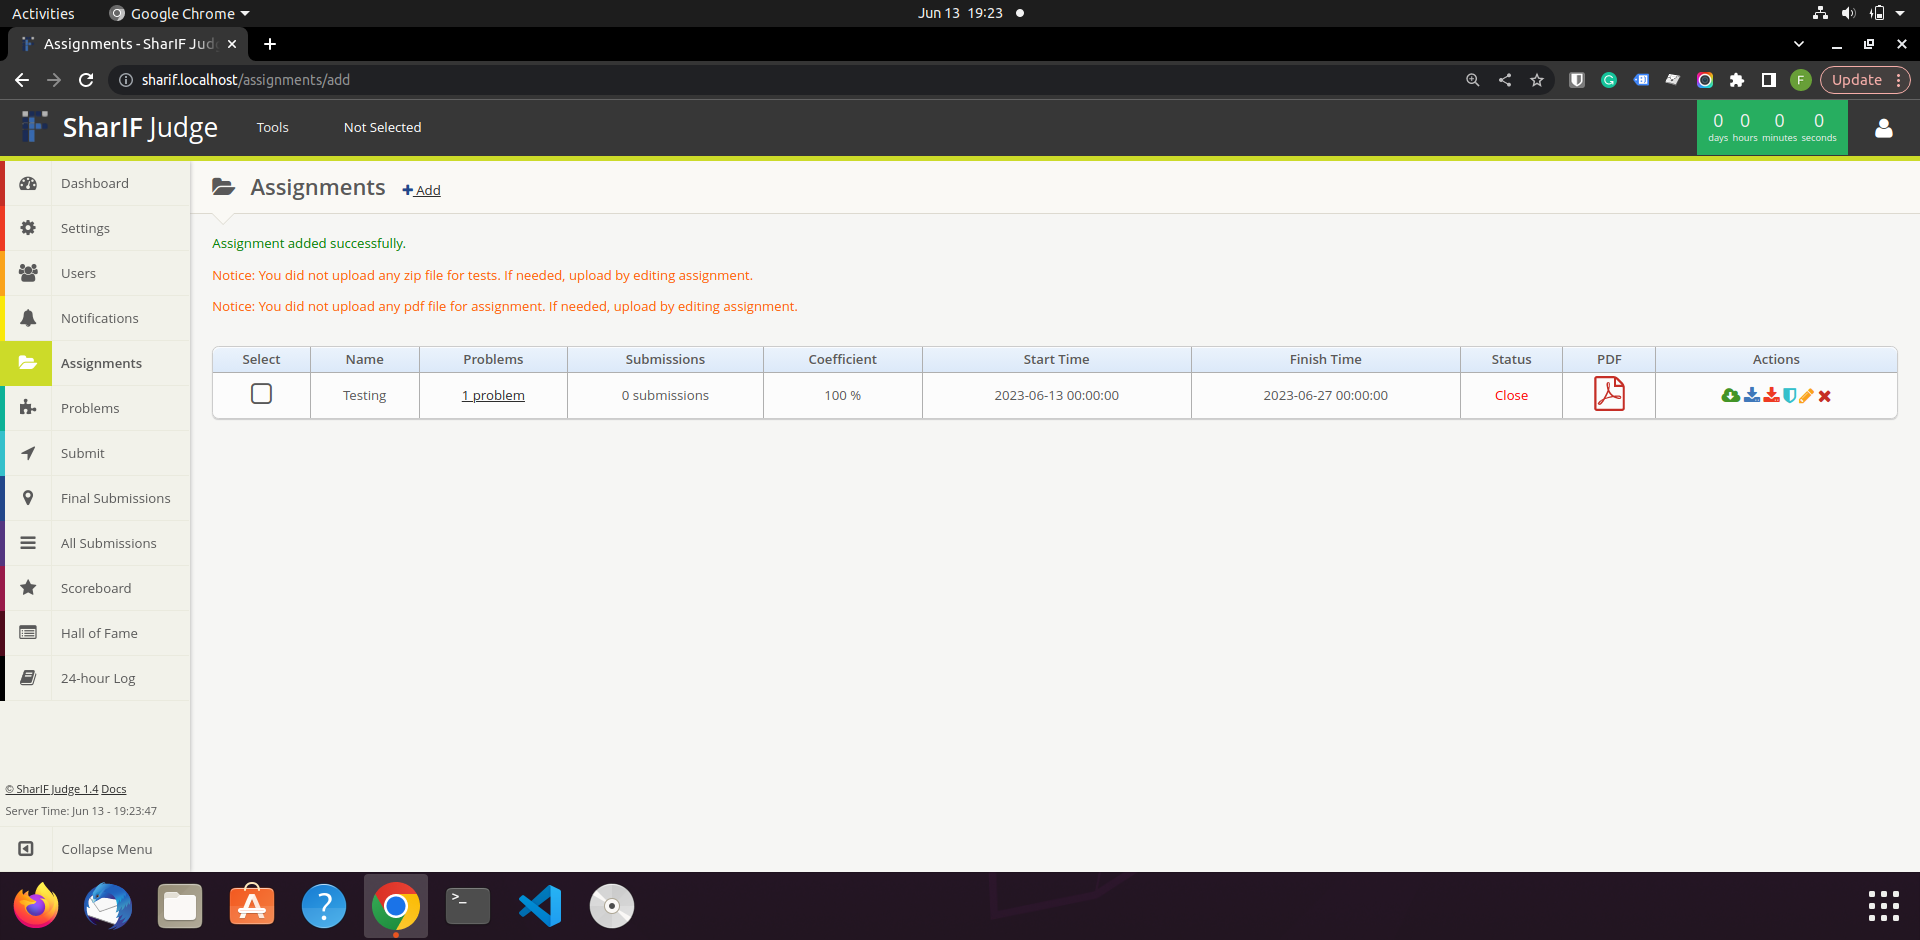
\includegraphics[scale=0.4]{assignments}  
	\caption[Tampilan Halaman \textit{Assignments}]{Tampilan Halaman Assignments} 
	\label{fig:assignments} 
\end{figure}

Gambar \ref{fig:assignments} merupakan tampilan halaman \textit{assignments} yang terdapat pada semua \textit{role} pengguna. Namun, terdapat bagian yang tidak dapat diakses oleh \textit{role} siswa dan \textit{instructor} yakni bagian \textit{actions}.
\subsubsection{\textit{Problems}}
\begin{figure}[H]
	\centering  
	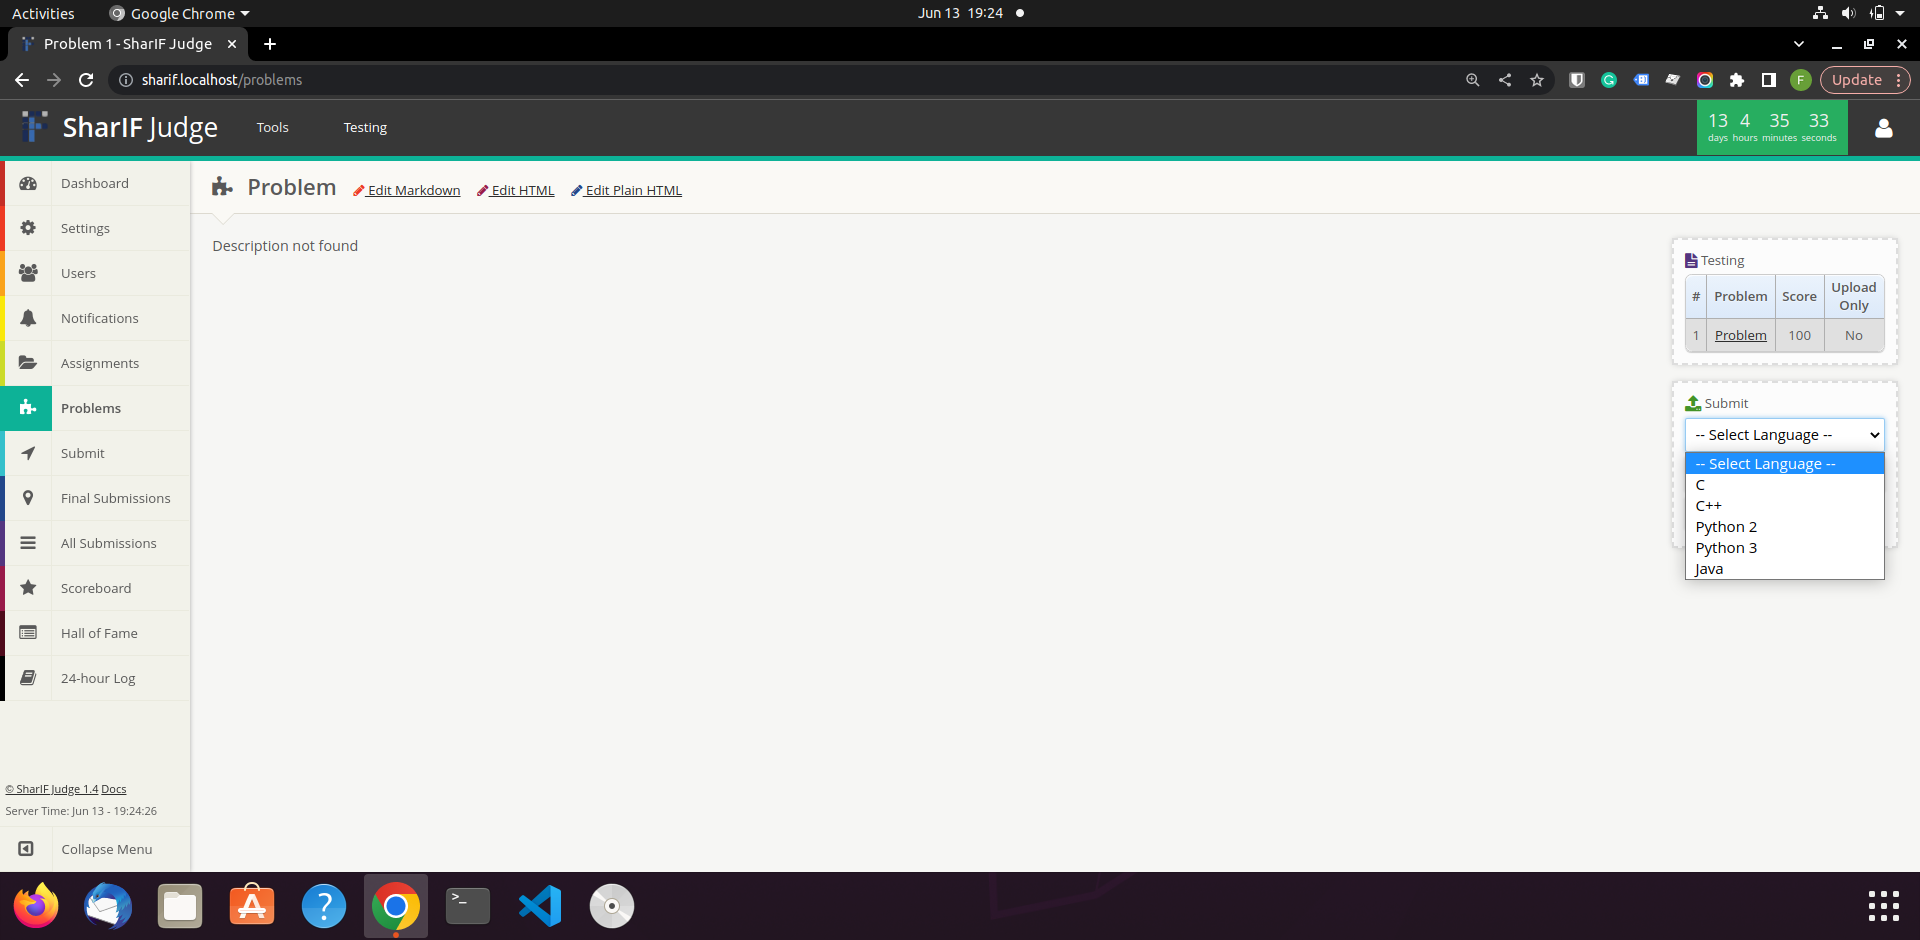
\includegraphics[scale=0.4]{problems}  
	\caption[Tampilan Halaman \textit{Problems}]{Tampilan Halaman Problems} 
	\label{fig:problems} 
\end{figure}

Gambar \ref{fig:problems} merupakan tampilan halaman \textit{problems} yang terdapat pada semua \textit{role} pengguna.

\subsubsection{\textit{Submit}}
\begin{figure}[H]
	\centering  
	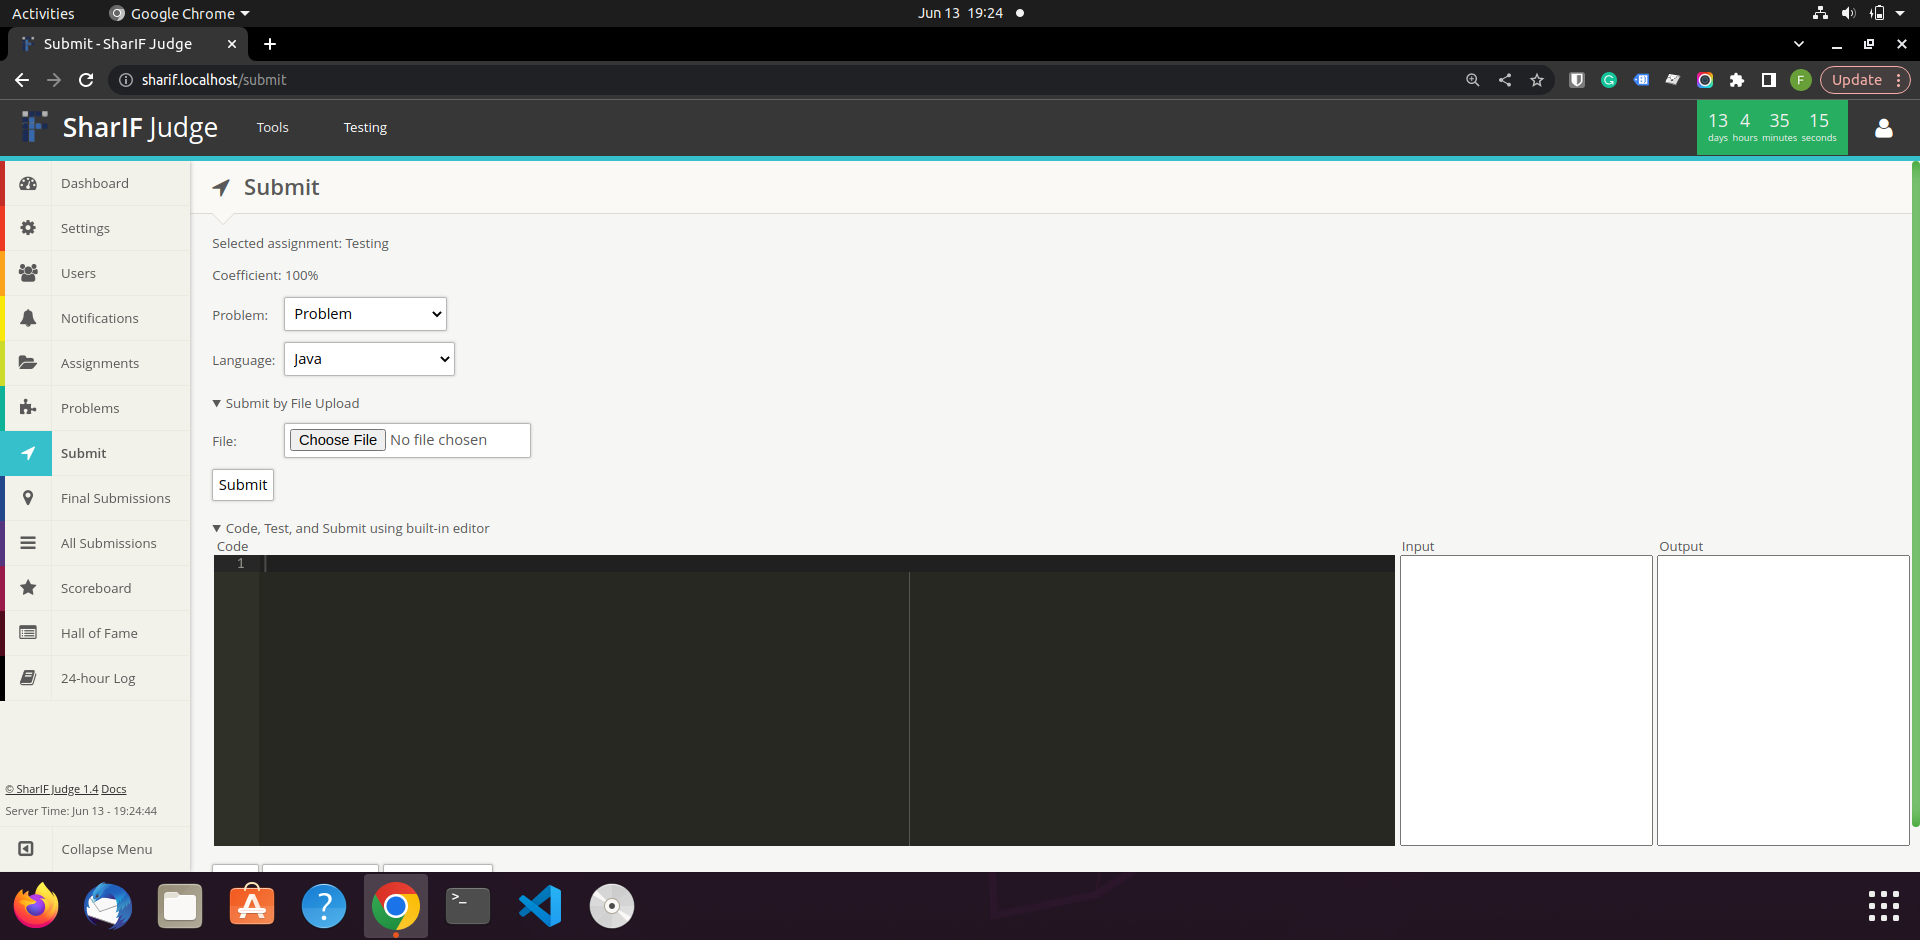
\includegraphics[scale=0.4]{submit}  
	\caption[Tampilan Halaman \textit{Submit}]{Tampilan Halaman Submit} 
	\label{fig:submit} 
\end{figure}

Gambar \ref{fig:submit} merupakan tampilan halaman \textit{submit} yang terdapat pada semua \textit{role} pengguna.

\subsubsection{\textit{Final Submissions}}
\begin{figure}[H]
	\centering  
	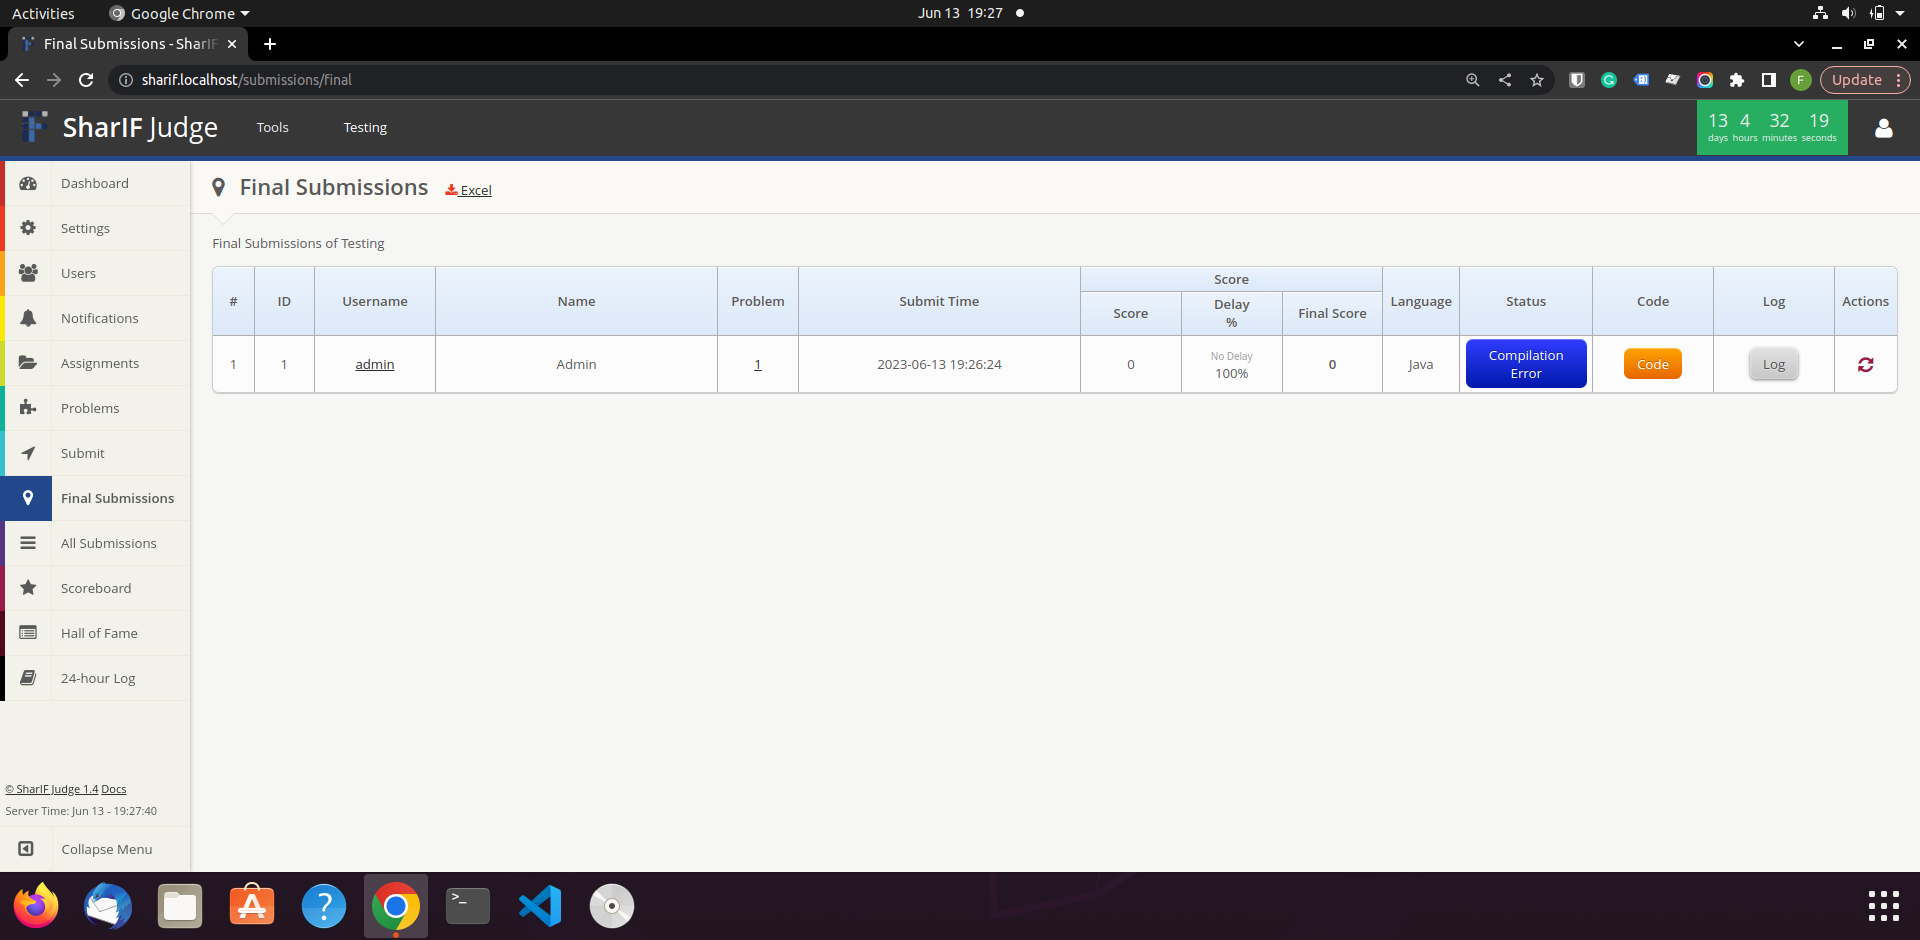
\includegraphics[scale=0.4]{finalsubmission}  
	\caption[Tampilan Halaman \textit{Final Submission}]{Tampilan Halaman Final Submission} 
	\label{fig:finalsubmission} 
\end{figure}

Gambar \ref{fig:finalsubmission} merupakan tampilan halaman \textit{submit} yang terdapat pada semua \textit{role} pengguna.
\subsubsection{\textit{All Submissions}}
\begin{figure}[H]
	\centering  
	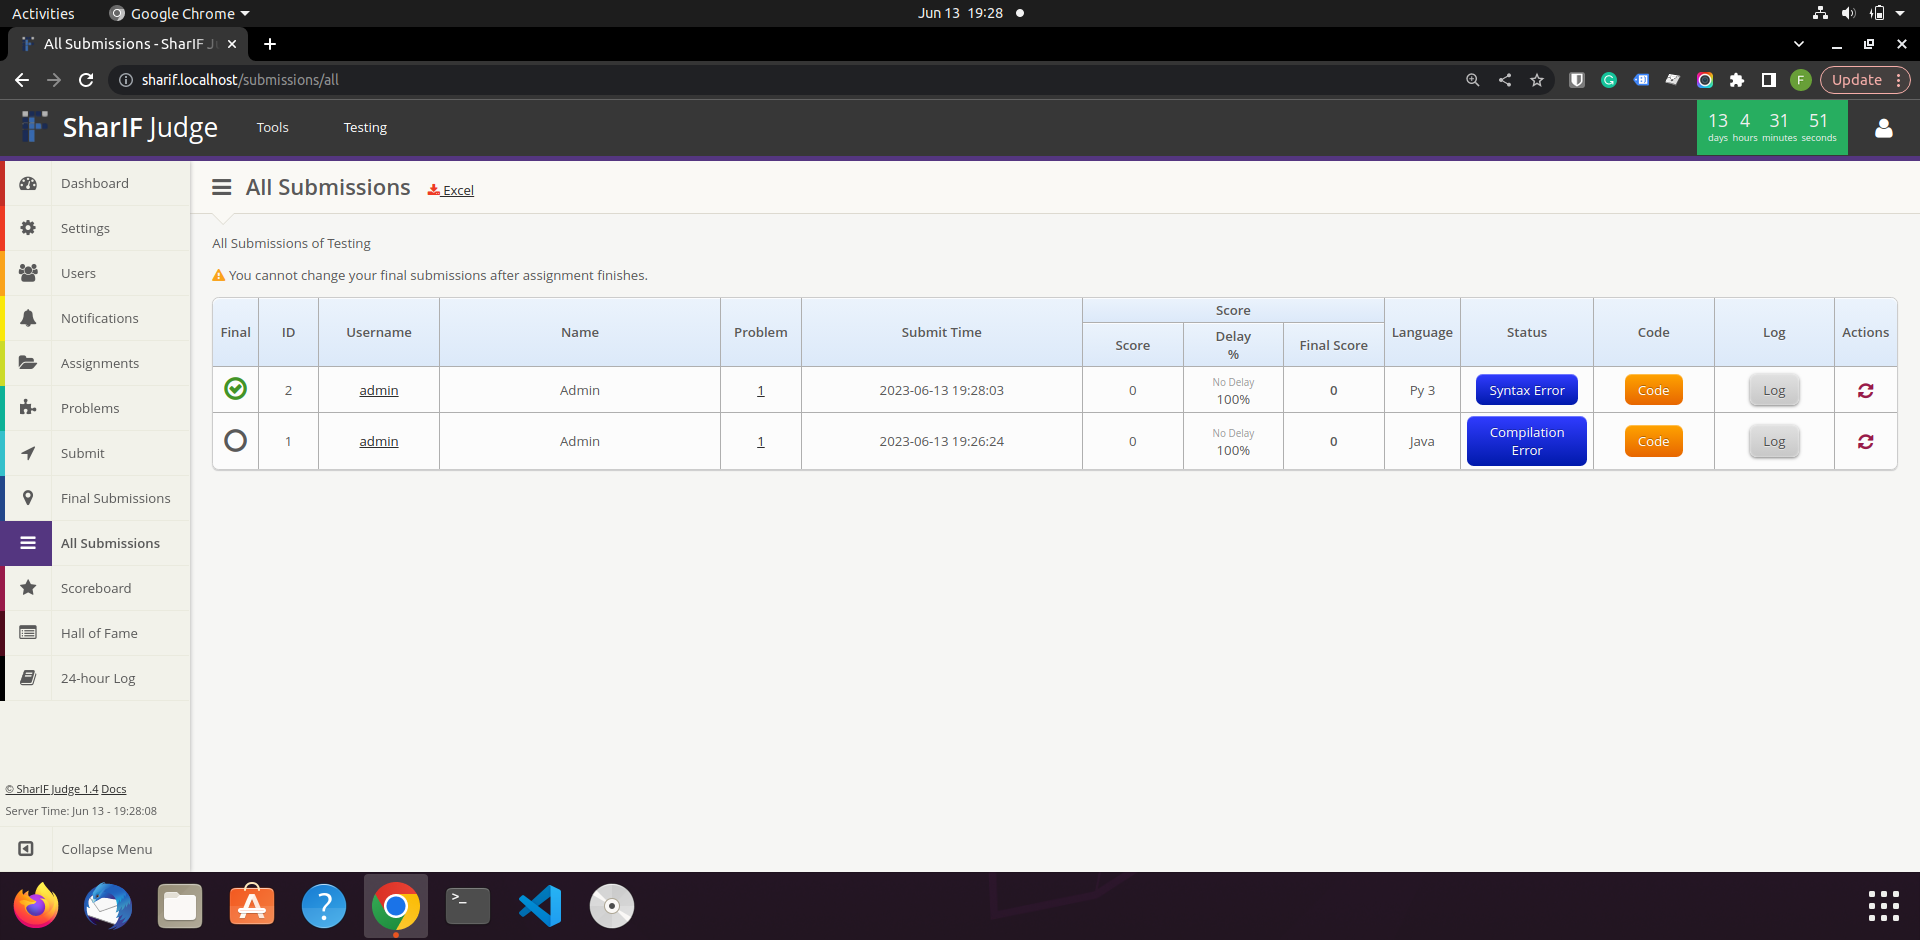
\includegraphics[scale=0.4]{allsubmission}  
	\caption[Tampilan Halaman \textit{All Submission}]{Tampilan Halaman All Submission} 
	\label{fig:allsubmission} 
\end{figure}

Gambar \ref{fig:allsubmission} merupakan tampilan halaman \textit{All Submission} yang terdapat pada semua \textit{role} pengguna.

\subsubsection{\textit{Scoreboard}}
\begin{figure}[H]
	\centering  
	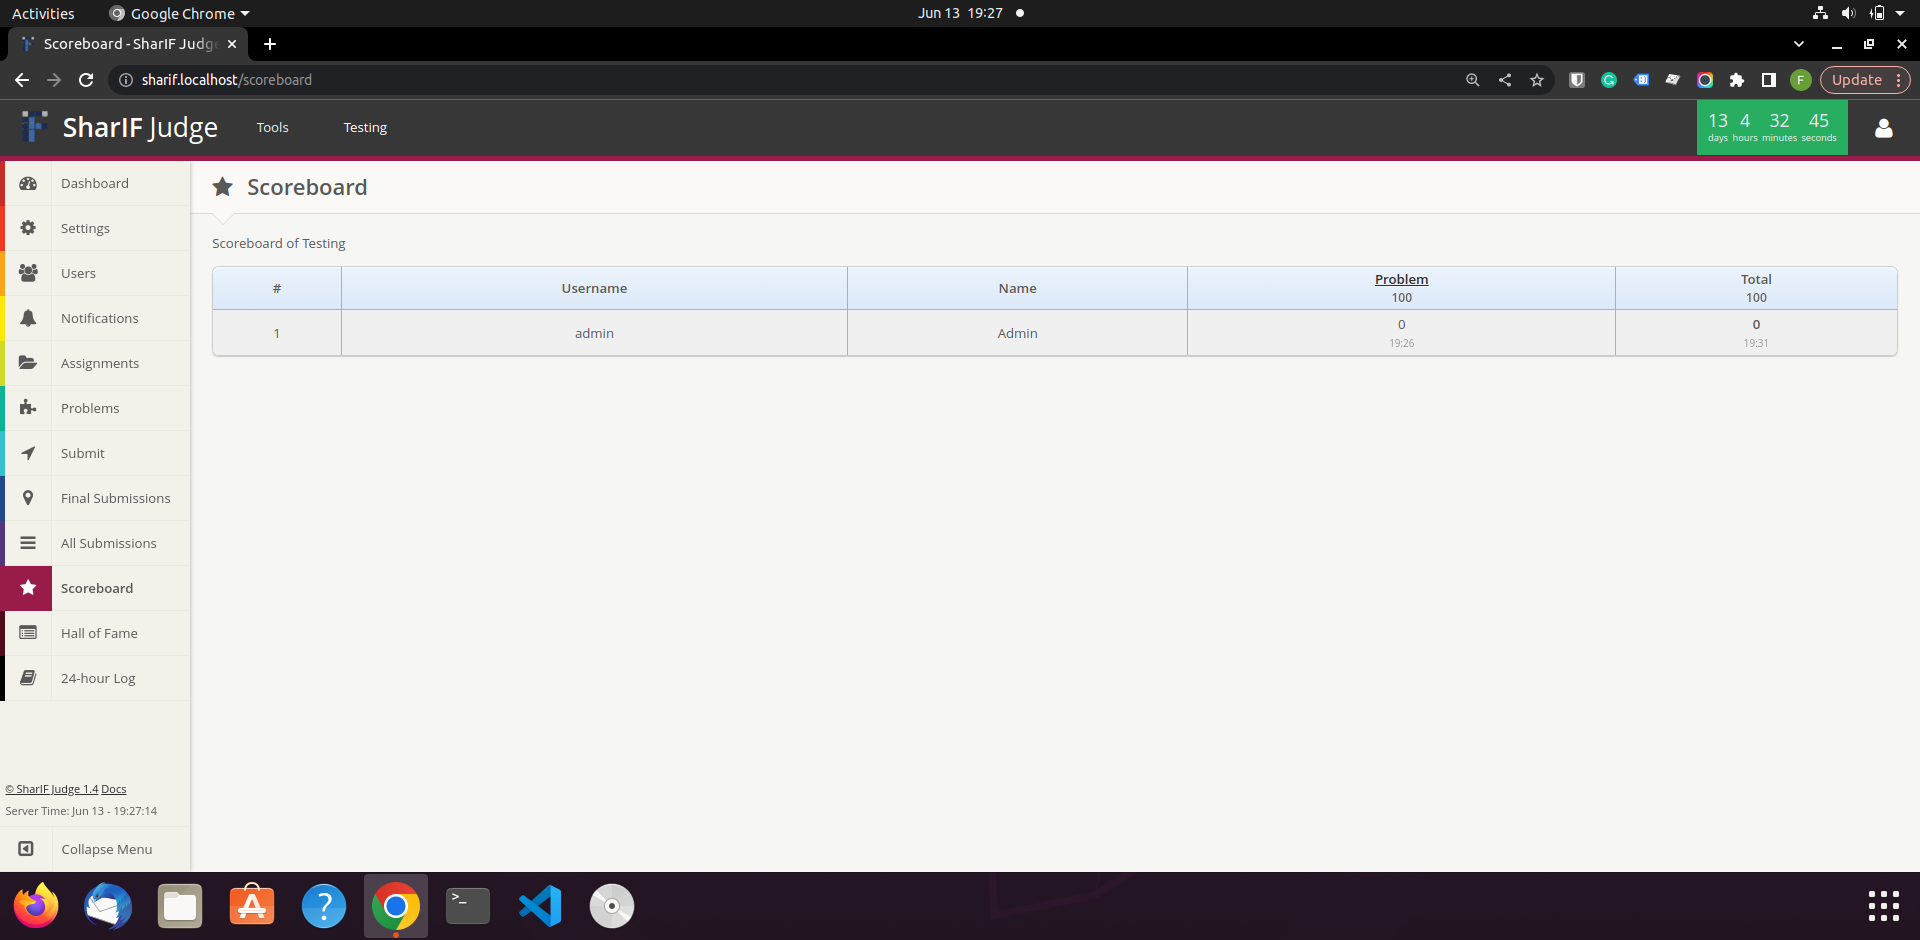
\includegraphics[scale=0.4]{scoreboard}  
	\caption[Tampilan Halaman \textit{Scoreboard}]{Tampilan Halaman Scoreboard} 
	\label{fig:scoreboard} 
\end{figure}

Gambar \ref{fig:allsubmission} merupakan tampilan halaman \textit{All Submission} yang terdapat pada semua \textit{role} pengguna.

\subsubsection{\textit{Hall of Fame}}
\begin{figure}[H]
	\centering  
	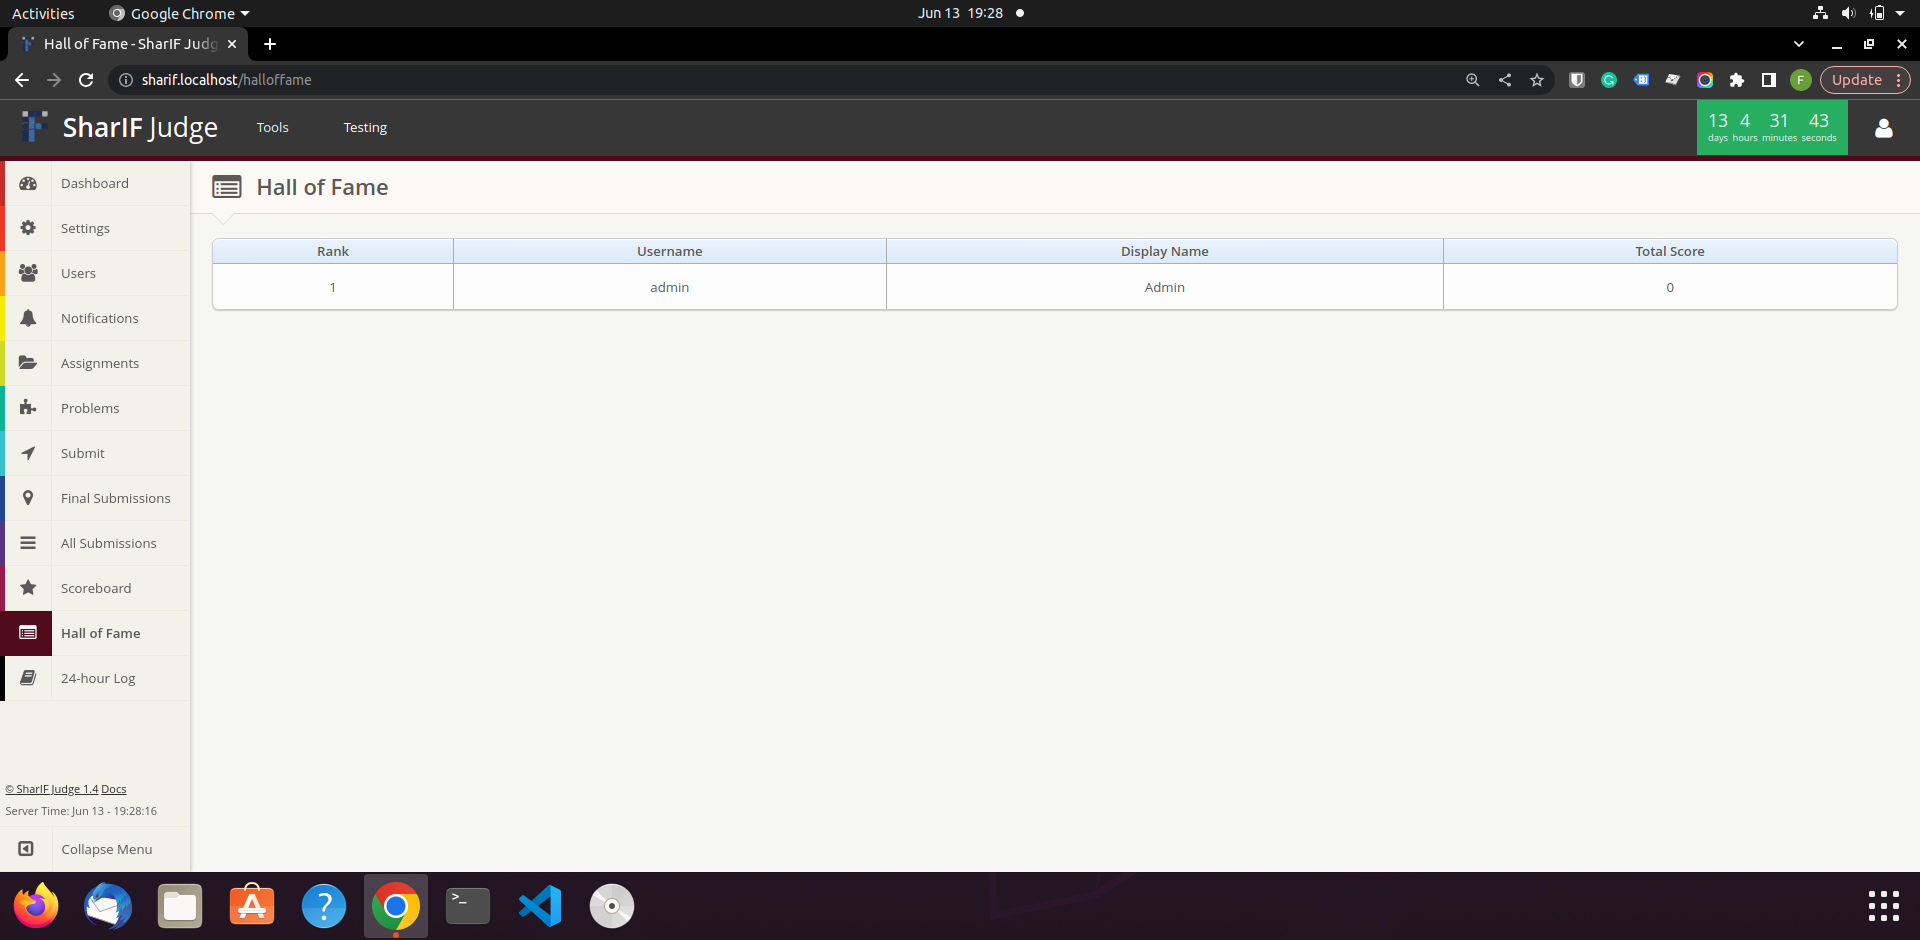
\includegraphics[scale=0.4]{halloffame}  
	\caption[Tampilan Halaman \textit{Hall of Fame}]{Tampilan Halaman Hall of Fame} 
	\label{fig:halloffame} 
\end{figure}

Gambar \ref{fig:halloffame} merupakan tampilan halaman \textit{Hall of Fame} yang terdapat pada semua \textit{role} pengguna.


\subsubsection{\textit{24-hour Log}}
\begin{figure}[H]
	\centering  
	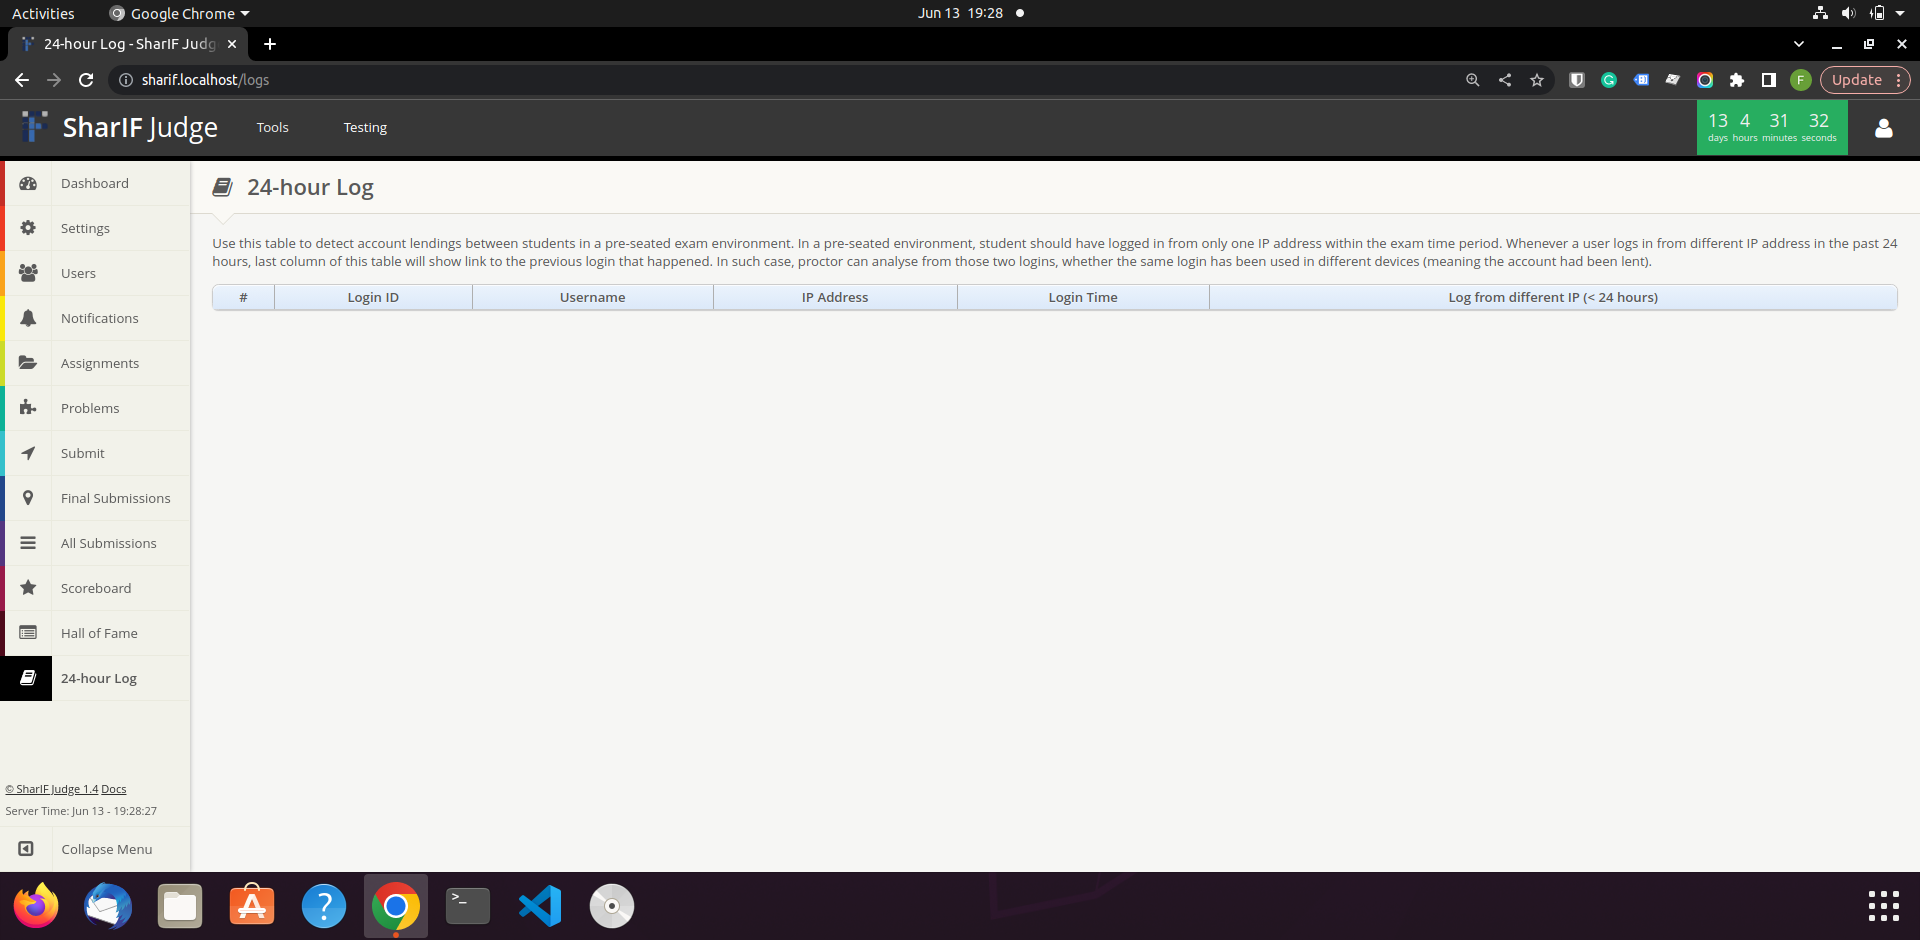
\includegraphics[scale=0.4]{24hourlog}  
	\caption[Tampilan Halaman \textit{24-hour Log}]{Tampilan Halaman 24-hour Log} 
	\label{fig:24hourlog} 
\end{figure}

Gambar \ref{fig:24hourlog} merupakan tampilan halaman \textit{24-hour Log} yang terdapat hanya pada \textit{role admin} dan \textit{head instructor}.

\subsubsection{\textit{Rejudge}}
\begin{figure}[H]
	\centering  
	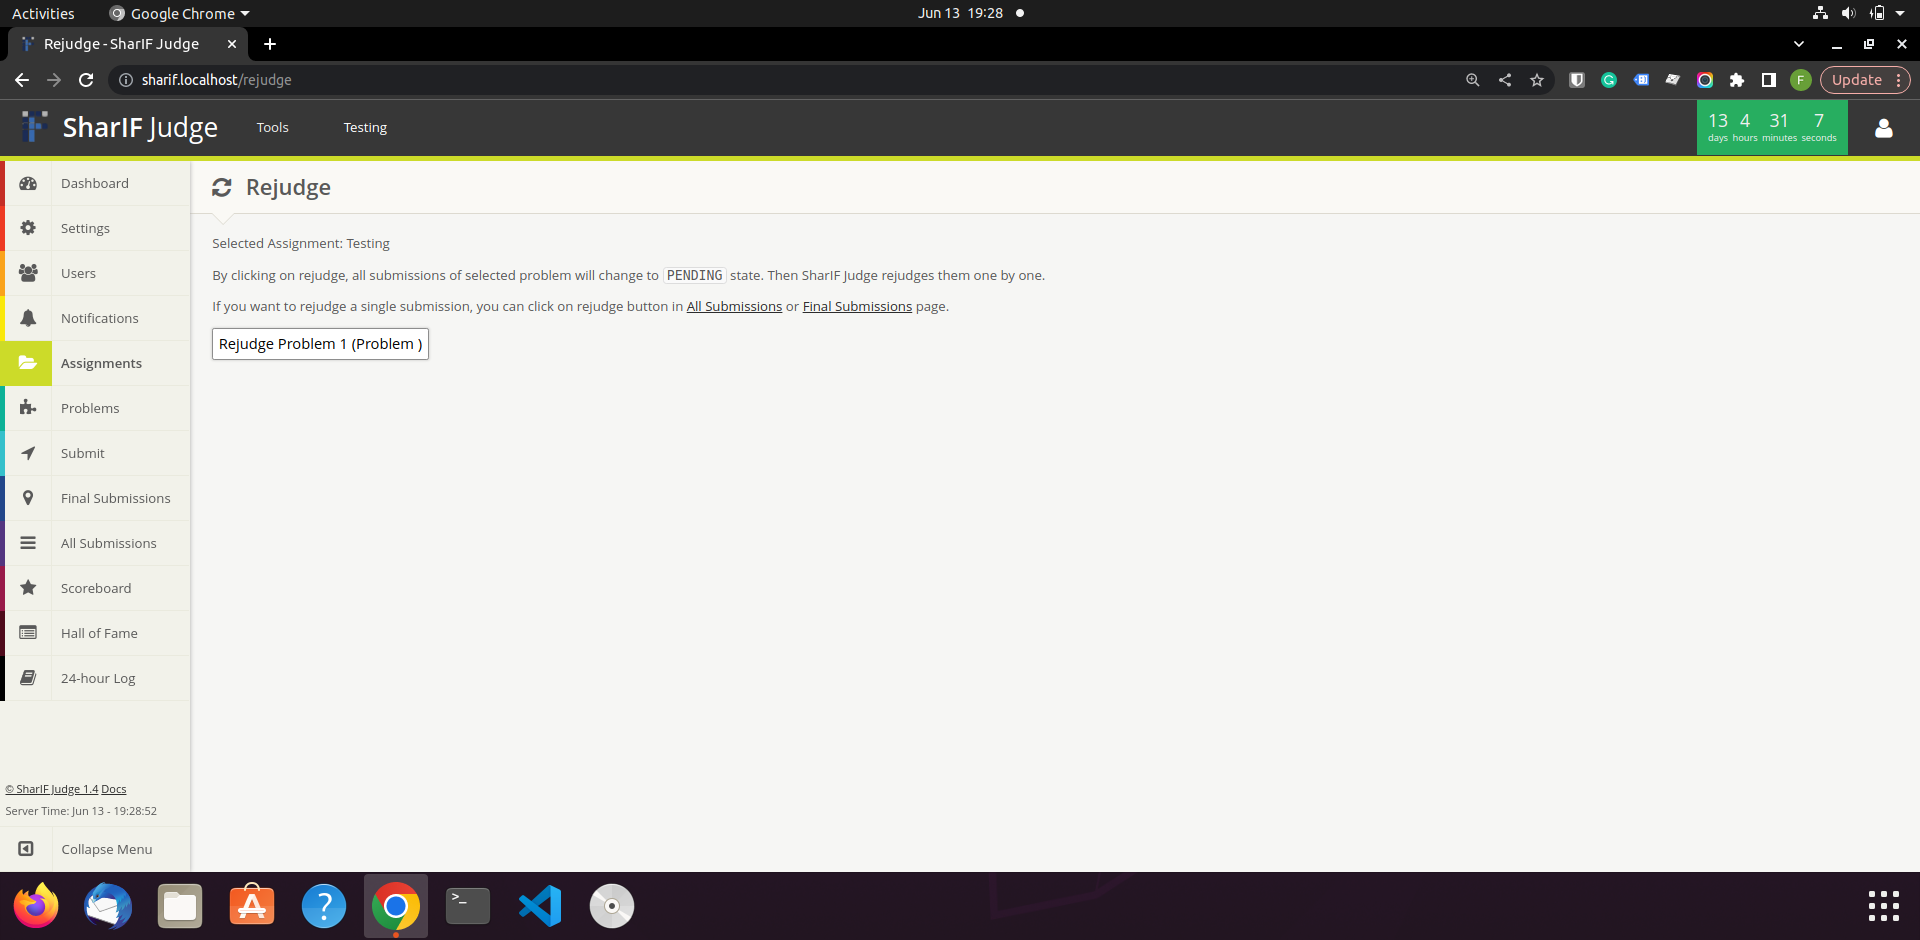
\includegraphics[scale=0.4]{rejudge}  
	\caption[Tampilan Halaman \textit{ReJudge}]{Tampilan Halaman ReJudge} 
	\label{fig:rejudge} 
\end{figure}

Gambar \ref{fig:rejudge} merupakan tampilan halaman \textit{ReJudge} yang terdapat hanya pada \textit{role admin} dan \textit{head instructor}.

\subsubsection{\textit{Submission Queue}}
\begin{figure}[H]
	\centering  
	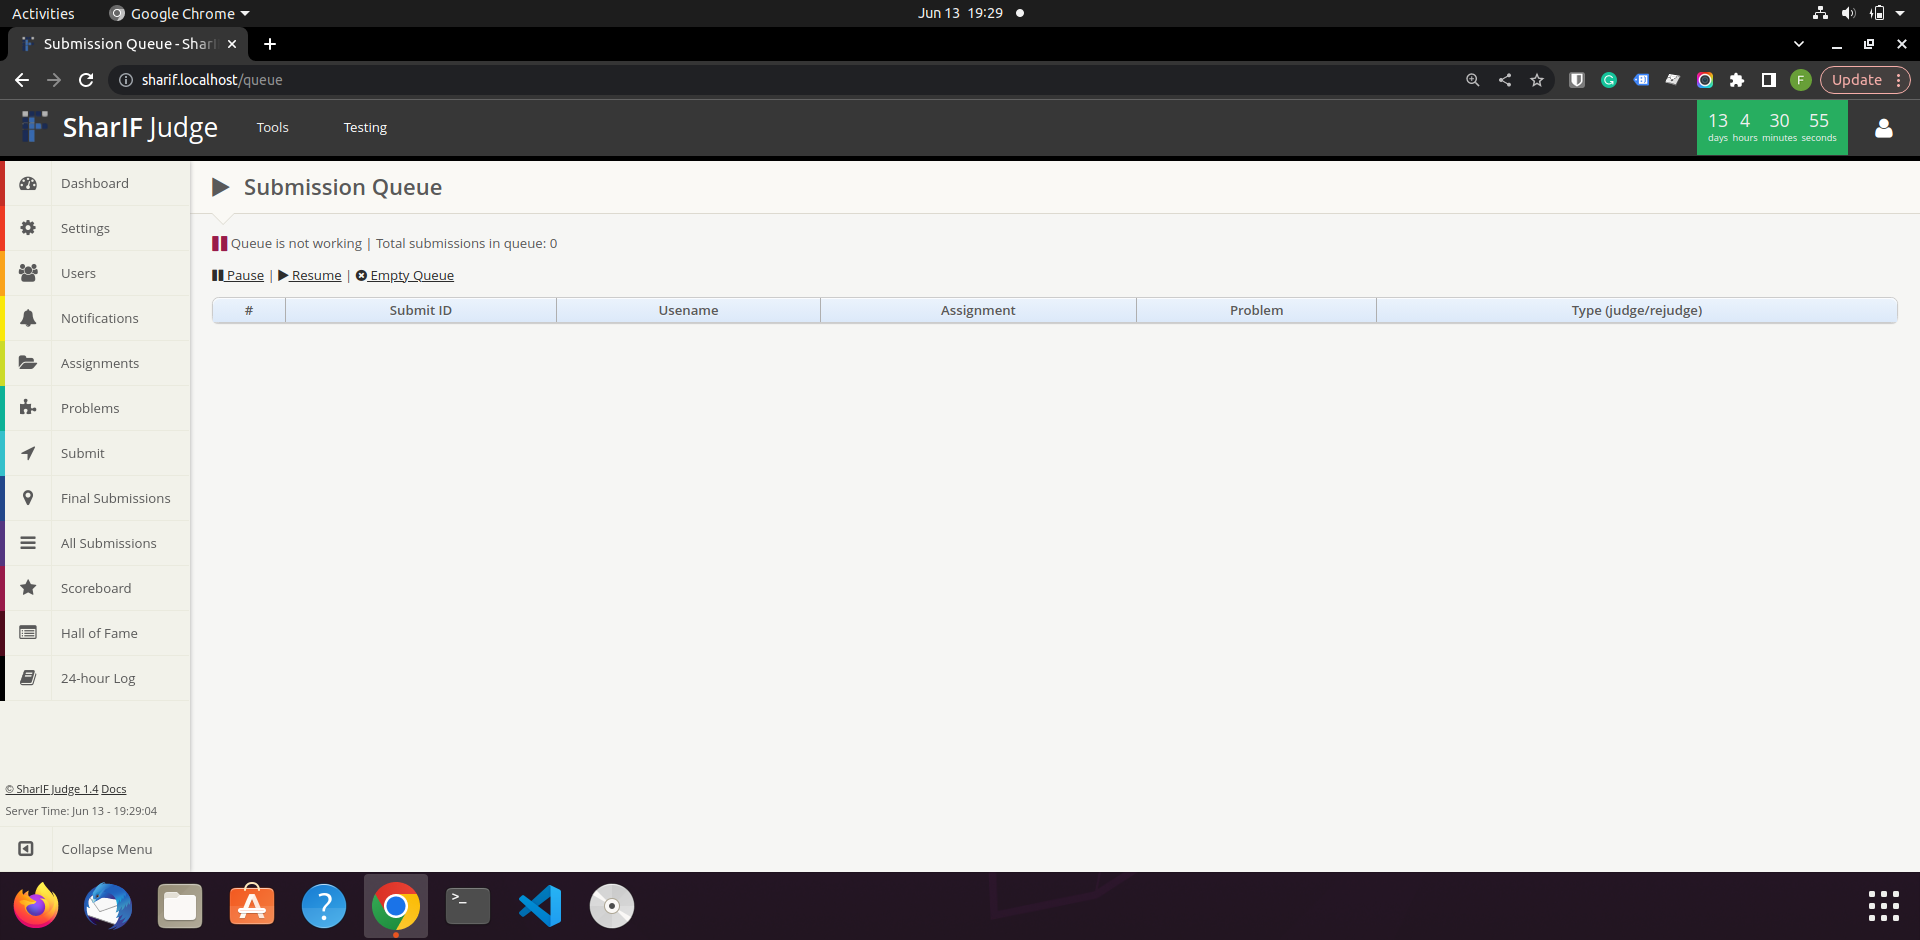
\includegraphics[scale=0.4]{submissionqueue}  
	\caption[Tampilan Halaman \textit{Submission Queue}]{Tampilan Halaman Submission Queue} 
	\label{fig:submissionqueue} 
\end{figure}

Gambar \ref{fig:submissionqueue} merupakan tampilan halaman \textit{Submission Queue} yang terdapat hanya pada \textit{role admin} dan \textit{head instructor}.

\subsubsection{\textit{Cheat Detection}}
\begin{figure}[H]
	\centering  
	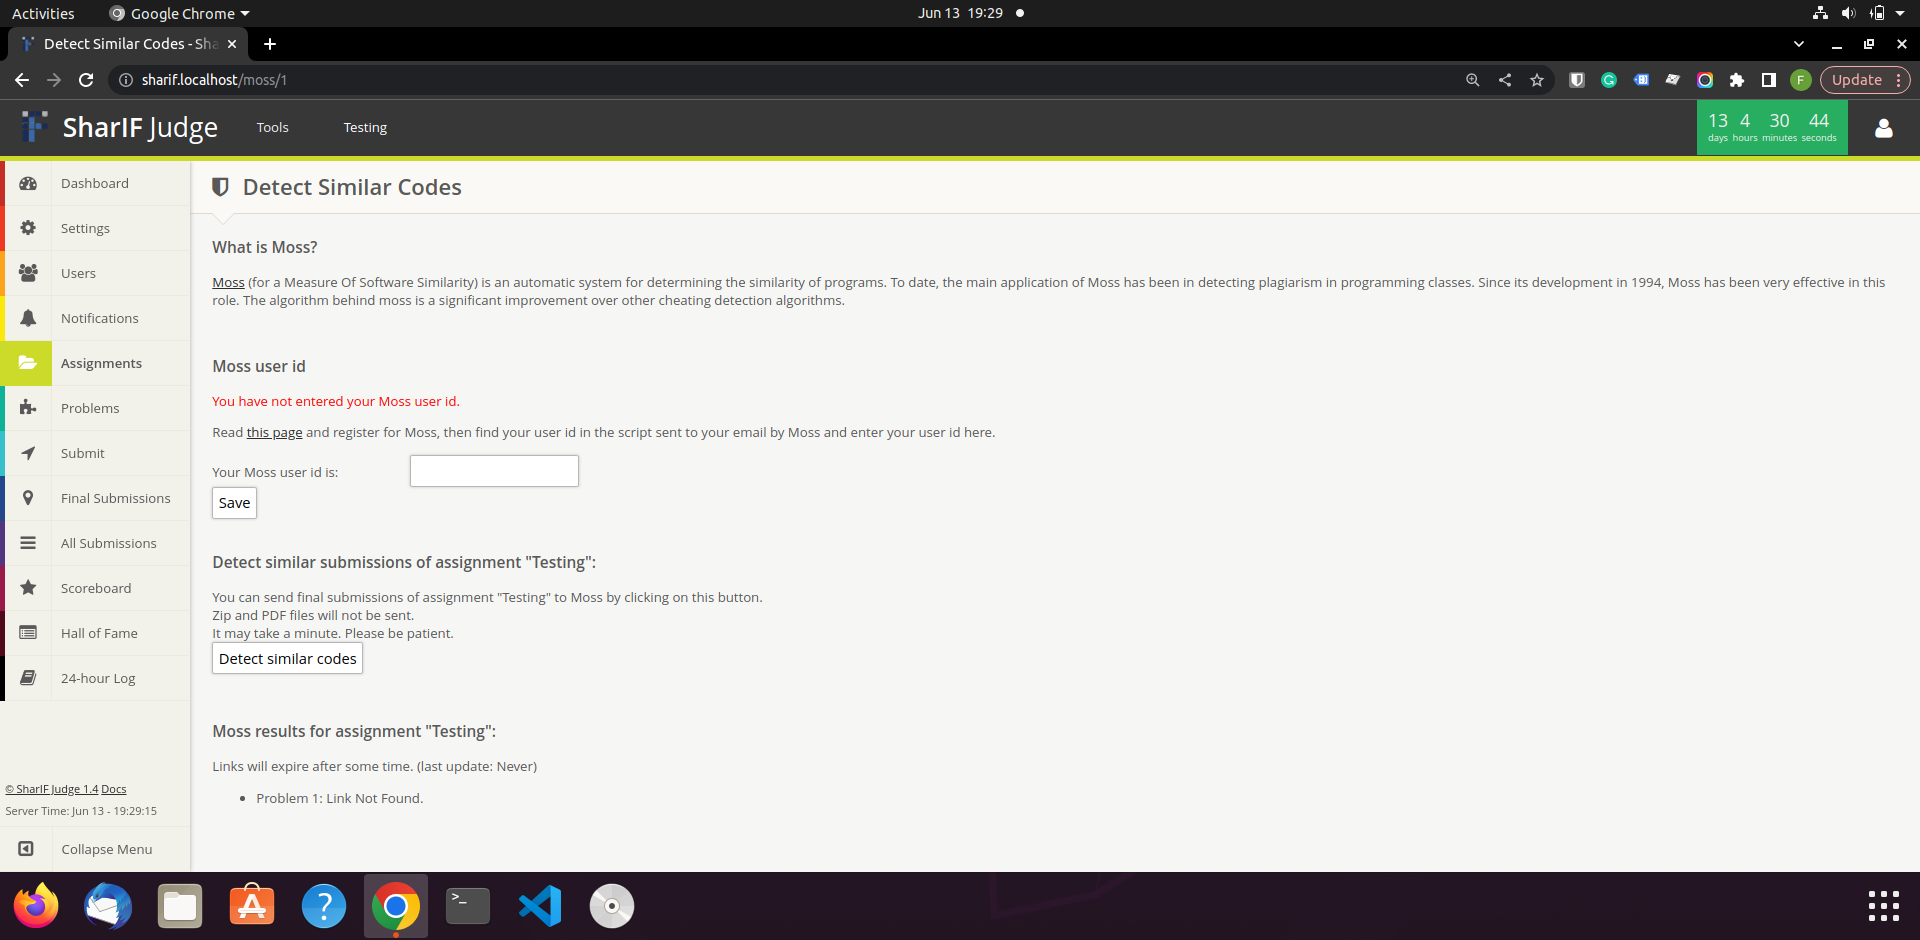
\includegraphics[scale=0.4]{cheatdetection}  
	\caption[Tampilan Halaman \textit{Cheat Detection}]{Tampilan Halaman Cheat Detection} 
	\label{fig:cheatdetection} 
\end{figure}

Gambar \ref{fig:cheatdetection} merupakan tampilan halaman \textit{Cheat Detection} yang terdapat hanya pada \textit{role admin} dan \textit{head instructor}.

\subsection{\textit{Controller}}
\textit{Controller} pada direktori \texttt{application/controller}. Direktori ini berisikan kelas \textit{controller} dengan fungsi-fungsi dalam mengambil atau memberikan data \textit{models} untuk dialihkan menuju \textit{views} untuk ditampilkan. Berikut merupakan \textit{controller} pada \textit{SharIF Jugde} beserta fungsi-fungsinya.
\subsubsection{\texttt{Assignments.php}}
Berikut merupakan fungsi-fungsi pada \textit{controller} \texttt{Assignments.php}.
\begin{itemize}
	\item \texttt{index}\\
	Fungsi ini berguna untuk mengambil dan memberikan data menuju halaman \texttt{assignments.twig} menggunakan \texttt{Assignment\_model}.
	\item \texttt{select}\\
	Fungsi ini berguna untuk memilih \textit{assignment} menggunakan \textit{ajax}.
	\item \texttt{pdf}\\
	Fungsi ini berguna untuk mengunduh \textit{assignment} atau \textit{problem} dalam bentuk pdf.
	\item \texttt{downloadtestsdesc}\\
	Fungsi ini berguna untuk mengunduh dan mengompres data \textit{test} dan deskripsi sebuah \textit{assignment}.
	\item \texttt{download\_submissions}\\
	Fungsi ini berguna untuk mengunduh dan mengompres kode terakhir sebuah \textit{assignment} pengguna.
	\item \texttt{delete}\\
	Fungsi ini berguna untuk menghapus \textit{assignment}.
	\item \texttt{add}\\
	Fungsi ini berguna untuk menambah atau mengubah \textit{assignment} berdasarkan masukan pengguna.
	\item \texttt{\_add}\\
	Fungsi ini berguna untuk menambah atau mengubah \textit{assignment}.
	\item \texttt{edit}\\
	Fungsi ini berguna untuk mengecek \textit{role} pengguna dapat mengubah \textit{assignment}. Selanjutnya akan dikembalikan pada fungsi \texttt{add}. 
	\item \texttt{pdfCheck}
	Fungsi ini berguna untuk mengecek \textit{file} pdf dari sebuah \textit{assignment}.
\end{itemize}

\subsubsection{\texttt{Dashboard.php}}
Berikut merupakan fungsi-fungsi pada \textit{controller} \texttt{Dashboard.php}.
\begin{itemize}
	\item \texttt{index}\\
	Fungsi ini berguna untuk mengambil dan memberikan data menuju halaman \textit{dashboard} menggunakan tiga buah \textit{model}. \textit{Model} tersebut terdiri dari \texttt{Assignment\_model}, \texttt{Settings\_model}, dan \texttt{Notifications\_model}.
	\item \texttt{widget\_positions}\\
	Fungsi ini berguna untuk menyimpan data \textit{widget} pengguna.
\end{itemize}
\subsubsection{\texttt{Install.php}}
\textit{Controller} \texttt{Install.php} hanya memiliki satu buah fungsi bernama \texttt{index}. Fungsi ini berguna untuk membentuk tabel yang dibutuhkan oleh \textit{SharIF Judge} pada \textit{database}. Selain itu, fungsi ini juga berguna untuk memasukan data pengguna \textit{admin} yang pertama kali memasang \textit{SharIF Judge} pada perangkat.

\subsubsection{\texttt{Login.php}}
Berikut merupakan fungsi-fungsi pada \textit{controller} \texttt{Login.php}.
\begin{itemize}
	\item \texttt{\_registration\_code}\\
	Fungsi ini beguna untuk memeriksa kode registrasi.
	\item \texttt{index}\\
	Fungsi ini berguna untuk melakukan validasi \textit{username} dan \textit{password} pengguna. Selain itu, fungsi ini juga memperbaharui \textit{log} pada tabel \textit{login}.
	\item \texttt{register}\\
	Fungsi ini berguna untuk melakukkan validasi dalam pembetukan akun.
	\item \texttt{logout}\\
	Fungsi ini berguna untuk menghancurkan \textit{session} dari pengguna dan memindahkan pengguna ke halaman \textit{login}.
	\item \texttt{lost}\\
	Fungsi ini berguna untuk mengirim \textit{email} lupa password.
	\item \texttt{rest}\\
	Fungsi ini berguna untuk melakukan \textit{reset password} pengguna.
\end{itemize}
\subsubsection{\texttt{Logs.php}}
\textit{Controller} \texttt{Logs.php} hanya memiliki satu buah fungsi bernama \texttt{index}. Fungsi ini berguna untuk mengambil dan memberikan data pada halaman \textit{logs} menggunakan \texttt{Logs\_model}.
\subsubsection{\texttt{Moss.php}}
Berikut merupakan fungsi-fungsi pada \textit{controller} \texttt{Moss.php}.
\begin{itemize}
	\item \texttt{index}\\
	Fungsi ini berguna untuk mengambil dan memberikan data pada halaman \textit{moss}.
	\item \texttt{update}\\
	Fungsi ini berguna untuk memperbaharui \textit{moss\_userid} yang dimasukan oleh pengguna.
	\item \texttt{\_detec}\\
	Fungsi ini berguna untuk melakukan pengecekan terhadap \textit{submission}. !!TODO
\end{itemize}
\subsubsection{\texttt{Notification.php}}
Berikut merupakan fungsi-fungsi pada \textit{controller} \texttt{Notification.php}.
\begin{itemize}
	\item \texttt{index}\\
	Fungsi ini berguna untuk mengambil dan memberikam data pada halaman \textit{notifications} menggunakan \texttt{assignment\_model} dan \texttt{notifications\_model}.
	\item \texttt{add}\\
	Fungsi ini berguna untuk menambahkan data \textit{notifications}.
	\item \texttt{edit}\\
	Fungsi ini berguna untuk memperbaharui data \textit{notifications}.
	\item \texttt{delete}\\
	Fungsi ini berguna untuk menghapus data \textit{notifications}.
	\item \texttt{check}\\
	Fungsi ini berguna memeriksa \textit{notifications} baru.
\end{itemize}
\subsubsection{\texttt{Problems.php}}
Berikut merupakan fungsi-fungsi pada \textit{controller} \texttt{Problems.php}.
\begin{itemize}
	\item \texttt{index}\\
	Fungsi ini berguna untuk mengambil dan memberikan data \textit{problems} sesuai dengan \textit{assignment} tertentu pada halaman \textit{problems}.
	\item \texttt{edit}\\
	Fungsi ini berguna untuk memperbaharui deskripsi \textit{problems} pada \textit{assignment} tertentu.
\end{itemize}
\subsubsection{\texttt{Profile.php}}
Berikut merupakan fungsi-fungsi pada \textit{controller} \texttt{Profile.php}.
\begin{itemize}
	\item \texttt{index}\\
	Fungsi ini berguna untuk mengambil dan memberikan data pada halaman \textit{profile}. Selain itu, fungsi ini berguna untuk melakukan pembaharuan data \textit{profile}.
	\item \texttt{\_password\_check}\\
	Fungsi ini berguna untuk melakukan validasi terhadap \textit{password} yang akan dimasukkan pengguna sesuai dengan aturan.
	\item \texttt{\_password\_again\_check}\\
	Fungsi ini berguna untuk melakukan validasi terhadap pengulangan \textit{password} yang dimasukkan pengguna.
	\item \texttt{\_email\_check}\\
	Fungsi ini berguna untuk melakukan validasi terhadap \textit{email} yang dimasukkan pengguna
	\item \texttt{\_role\_check}\\
	 Fungsi ini berguna untuk melakukan validasi \textit{role} pengguna.
\end{itemize}
\subsubsection{\texttt{Queue.php}}
\begin{itemize}
	\item \texttt{index}\\
	Fungsi ini berguna untuk mengambil dan meberikan data pada halaman \textit{queue} menggunakan tiga buah \textit{model}. \textit{Model} tersebut adalah \texttt{Assignment\_model}, \texttt{queue\_model}, dan \texttt{settings\_model}.
	\item \texttt{pause}\\
	Fungsi ini berguna untuk memperbaharui data pada tabel \textit{settings}.
	\item \texttt{resume}\\
	Fungsi ini berguna untuk melanjutkan proses \textit{queue}.
	\item \texttt{empty\_queue}\\
	Fungsi ini berguna untuk menghapus data tabel \textit{queue}.
\end{itemize}
\subsubsection{\texttt{Queueprocess.php}}
\textit{Controller} \texttt{Queueprocess.php} hanya memiliki satu buah fungsi bernama \texttt{index}.Fungsi ini berguna untuk menjalankan proses \textit{judge} berdasarkan \textit{queue} satu demi satu sesuai antrean. Fungsi ini menggunakan beberapa \textit{model} yaitu \texttt{Queue\_model}, \texttt{Submit\_model}, \texttt{Assignments\_model}, dan \texttt{Settings\_model}.
\subsubsection{\texttt{Rejudge.php}}
Berikut merupakan fungsi-fungsi pada \textit{controller} \texttt{Rejudge.php}.
\begin{itemize}
	\item \texttt{index}\\
	Fungsi ini berguna untuk mengambil dan memberikan data pada halaman \textit{rejudge} menggunakan \texttt{Assignment\_model}.
	\item \texttt{rejudge\_single}\\
	Fungsi ini berguna untuk melakukan \textit{rejudge} pada satu buah masalah tertentu.
\end{itemize}
\subsubsection{\texttt{Scoreboard.php}}
Berikut merupakan fungsi-fungsi pada \textit{controller} \texttt{Scoreboard.php}.
\begin{itemize}
	\item \texttt{index}\\
	Fungsi ini berguna untuk memberikan data pada halaman \textit{scoreboard} menggunakan dua buah \textit{model}. \textit{Model} tersebut adalah \texttt{Assignment\_model} dan \texttt{Scoreboard\_model}.
\end{itemize}
\subsubsection{\texttt{Server\_time.php}}
\textit{Controller} \texttt{Server\_time.php} hanya memiliki satu buah fungsi bernama \texttt{index}. Fungsi ini berguna untuk mengeluarkan \textit{server\_time}.

\subsubsection{\texttt{Settings.php}}
Berikut merupakan fungsi-fungsi pada \textit{controller} \texttt{Settings.php}.
\begin{itemize}
	\item \texttt{index}\\
	Fungsi ini berguna untuk mengambil dan memberikan data pada halaman \textit{settings} menggunakan \texttt{Settings\_model} dan \texttt{Assignment\_model}.
	\item \texttt{update}\\
	Fungsi ini berguna untuk mengambil masukan dan memperbaharui data pada halaman \textit{settings} berdasarkan masukan tersebut. Data tersebut nantinya akan disimpan pada \textit{database} menggunakan fungsi \texttt{Settings\_model}.  
\end{itemize}
\subsubsection{\texttt{Submission.php}}
Berikut merupakan fungsi-fungsi pada \textit{controller} \texttt{Submission.php}.
\begin{itemize}
	\item \texttt{\_download\_excel}\\
	Fungsi ini berguna untuk mengubah data-data dari \textit{submission} yang dipilih menjadi format \textit{excel}.
	\item \texttt{final\_excel}\\
	Fungsi ini berguna untuk mengunduh data \textit{final submissions}.
	\item \texttt{all\_excel}\\
	Fungsi ini berguna untuk mengunduh data seluruh \textit{submissions}.
	\item \texttt{the\_final}\\
	Fungsi ini berguna untuk memberikan data pada halaman \textit{Final Submissions} menggunakan beberapa \textit{model}. \textit{Model} tersebut terdiri dari \texttt{Submit\_model}, \texttt{Settings\_model}, dan \texttt{User\_model}.
	\item \texttt{all}\\
	Fungsi ini berguna untuk memberikan data pada halaman \textit{All Submissions} menggunakan beberapa \textit{model}. \textit{Model} tersebut terdiri dari \texttt{Submit\_model}, \texttt{Settings\_model}, dan \texttt{User\_model}.
	\item \texttt{select}\\
	Fungsi ini berguna untuk memilih \textit{submission} yang akan dijadikan \textit{submission final} oleh pengguna.
	\item \texttt{\_check\_type}\\
	Fungsi ini berguna untuk melakukan pengecekan tipe \textit{submission} yang telah dikumpulkan oleh pengguna.
	\item \texttt{view\_code}\\
	Fungsi ini berguna untuk memperlihatkan \textit{submission} yang telah dikumpulkan oleh pengguna sesuai dengan tipenya.
	\item \texttt{download\_file}\\
	Fungsi ini berguna untuk mengunduh hasil dari \textit{submission} yang telah dikumpulkan oleh pengguna.
\end{itemize}
\subsubsection{\texttt{Submit.php}}
Berikut merupakan fungsi-fungsi pada \textit{controller} \texttt{Submit.php}.
\begin{itemize}
	\item \texttt{\_language\_to\_type}\\
	Fungsi ini berguna untuk mengubah bahasa pemrograman menjadi tipe sesuai dengan pilihan pengguna.
	\item \texttt{\_language\_to\_ext}\\
	Fungsi ini berguna untuk mengubah bahasa pemrograman menjadi ekstensi sesuai dengan pilihan pengguna.
	\item \texttt{\_match}\\
	Fungsi ini berguna untuk mencocokan tipe dengan ekstensi dari bahasa pemrogramannya.
	\item \texttt{\_check\_language}\\
	Fungsi ini berguna untuk melakukan pengecekan terhadap bahasa pemrograman yang digunakan.
	\item \texttt{index}\\
	Fungsi ini berguna untuk mengambil dan memberikan data pada halaman \textit{submit} menggunakan \texttt{Assignment\_model}. 
	\item \texttt{\_upload}\\
	Fungsi ini berguna untuk menyimpan jawaban dan memasukannya ke \textit{queue} untuk dinilai.
	\item \texttt{load}\\
	Fungsi ini berguna untuk memuat kode dari \textit{editor file}.
	\item \texttt{save}\\
	Fungsi ini berguna untuk meyimpan kode menuju \textit{editor file} dan mengirim ataupun menjalankannya.
	\item \texttt{\_submit}\\
	Fungsi ini berguna untuk menambahkan kode pada \textit{queue} untuk dilakukan \textit{judge}.
	\item \texttt{\_execute}\\
	Fungsi ini berguna untuk menambahkan kode untuk dijalankan atau di \textit{queue}.
	\item \texttt{get\_output}
	Fungsi ini berguna untuk memuat \textit{file} menjadi hasil eksekusi.
\end{itemize}
\subsubsection{\texttt{User.php}}
Berikut merupakan fungsi-fungsi pada \textit{controller} \texttt{User.php}.
\begin{itemize}
	\item \texttt{index}\\
	Fungsi ini berguna untuk mengambil dan memberikan data pada halaman \textit{users}.
	\item \texttt{add}\\
	Fungsi ini berguna untuk menambahkan pengguna baru sesuai dengan masukan.
	\item \texttt{delete}\\
	Fungsi ini berguna untuk menghapus pengguna yang dipilih.
	\item \texttt{delete\_submissions}\\
	Fungsi ini berguna untuk menghapus \textit{submission} dari sebuah pengguna.
	\item \texttt{list\_excel}\\
	Fungsi ini berguna untuk menghasilkan dan mengunduh data pengguna pada format \textit{excel}.
\end{itemize}

\subsection{\textit{Assets}}
Direktori ini berisikan seluruh kebutuhan pengguna seperti \textit{library javascript} dan juga gambar yang akan ditampilkan pada aplikasi. Berikut merupakan isi dari direktori ini beserta kegunaannya.
\begin{itemize}
	\item Direktori \textit{ace} \\ Direktori ini berisikan \textit{javascript} yang berfungsi untuk menambahkan \textit{code editor} pada aplikasi.
	\item Direktori \textit{font} \\Direktori ini berisikan seluruh \textit{font} yang digunakan oleh aplikasi \textit{SharIF Jugde}.
	\item Direktori \textit{fullcalendar} \\Direktori ini berisikan \textit{javascript} dan \textit{css} yang berfungsi untuk menambahkan kalender pada aplikasi.
	\item Direktori \textit{gridster} \\Direktori ini berisikan \textit{javascript}, \textit{css}, dan gambar yang berfungsi untuk membentuk kolom \textit{grid} dengan sifat \textit{drag and drop}.
	\item Direktori \textit{images} \\Direktori ini berisikan seluruh gambar yang digunakan pada aplikasi \textit{SharIF Judge} seperti banner dan juga logo.
	\item Direktori \textit{js} \\Direktori ini berisikan \textit{javascript} dan \textit{jquery}. \textit{Javascript} dan \textit{jquery} yang terdapat pada direktori ini dibentuk secara manual dan diambil dari situs resmi.
	\item Direktori \textit{nano\_scroller} \\Direktori ini berisikan \textit{jquery} dan \textit{css} yang berfungsi untuk membentuk \textit{scrollbar} pada aplikasi.
	\item Direktori \textit{noty} \\Direktori ini berisikan \textit{javascript} yang berfungsi untuk mempermudah membentuk pesan \textit{alert, success,} dan sebagainya.
	\item Direktori \textit{pdfjs} \\Direktori ini berisikan \textit{javascript} yang berfungsi untuk melakukan \textit{parsing} dan \textit{rendering} file \textit{pdf}.
	\item Direktori \textit{reveal} \\Direktori ini berisikan \textit{jquery} dan \textit{css} yang berfungsi untuk menampilkan \textit{popup} berupa halaman yang dikonfigurasikan.
	\item Direktori \textit{snippet} \\Direktori ini berisikan \textit{javascript} dan \textit{css} yang berfungsi sebagai \textit{template} dalam membentuk kode \textit{javascript}.
	\item Direktori \textit{styles} \\Direktori ini berisikan \textit{css} yang berfungsi untuk memperindah aplikasi yang dibentuk.
	\item Direktori \textit{tinymce} \\Direktori ini berisikan \textit{javascript} dan \textit{css} yang berfungsi untuk membentuk \textit{WYSIWYG editor} pada sebuah aplikasi.
\end{itemize}

\subsection{\textit{Libraries}}
\textit{SharIF Judge} menggunakan beberapa \textit{library} yang dibentuk secara manual maupun yang sudah tersedia pada \textit{Codeigniter 3}. Berikut merupakan \textit{library} yang dipakai oleh \textit{SharIF Judge}:

\subsubsection{\textit{Unzip}}
\textit{Unzip} merupakan sebuah \textit{library} yang dibentuk oleh Phil Sturgeon. \textit{Library} ini mewajibkan pengguna untuk menyalakan \textit{extension Zlib} sebelum dapat digunakan. \textit{Library Unzip} berfungsi untuk mengextraksi file dengan \textit{extension} \texttt{.zip} menuju direktori yang ditentukan dan dapat mengeluarkan \textit{error} yang sesuai. \textit{Library} ini juga dapat memberi batasan \textit{extension} apa yang diinginkan dari file tersebut. Kode \ref{kode:unzipsharif} merupakan contoh penggunaan \textit{library Unzip} pada \textit{SharIF Judge}.

\begin{lstlisting}[caption=Contoh kode penggunaan \textit{Library Unzip}, label=kode:unzipsharif]
	$this->load->library('unzip');
	$this->unzip->allow(array('txt', 'cpp', 'html', 'md', 'pdf'));
	$extract_result = $this->unzip->extract($u_data['full_path'], $tmp_dir);
\end{lstlisting}

Kode \ref{kode:unzipsharif} merupakan contoh penggunakan \textit{library Unzip}. Sintaks \verb|$this->load->library('unzip');| berfungsi untuk melakukan \textit{load} \textit{library Unzip} agar dapat digunakan pada fungsi tersebut. Selanjutnya sintaks \verb|$this->unzip->allow(array('txt', 'cpp', 'html', 'md', 'pdf'));| berfungsi untuk memberikan batasan \textit{extension} apa saja yang diinginkan dari file tersebut. Terakhir sintaks \verb|$extract_result = $this->unzip->extract($u_data['full_path'], $tmp_dir);| berfungsi untuk melakukan ekstraksi terhadap file zip pada \verb|$u_data['full_path']| tersebut menuju direktori pada variabel tmp\_dir.

\subsubsection{\textit{Twig}}
\textit{Twig} merupakan sebuah \textit{template engine library} yang digunakan untuk mempermudah dalam membentuk \textit{view} pada aplikasi. \textit{Twig} terintegrasi dengan fungsi-fungsi pada \textit{CodeIgniter 3} sehingga dapat menggunakan seluruh fungsi yang terdapat pada \textit{CodeIgniter 3}. Kode \ref{kode:twigsharif} merupakan contoh penggunaan \textit{Twig} pada \textit{SharIF Judge}.
\begin{lstlisting}[caption=Contoh \textit{view} menggunakan \textit{library Twig}, label=kode:twigsharif]



{{ form_open() }}
	<div class="box login">

		<div class="judge_logo">
			<a href="{{ site_url() }}"><img src="{{ base_url('assets/images/banner.png') }}"/></a>
		</div>

		<div class="login_form">
			<div class="login1">
				<p>
					<label for="form_username">Username</label><br/>
					<input id="form_username" type="text" name="username" required="required" pattern="[0-9a-z]{3,20}" title="The Username field must be between 3 and 20 characters in length, and contain only digits and lowercase letters" class="sharif_input" value="{{ set_value('username') }}" autofocus="autofocus"/>
					{{ form_error('username', '<div class="shj_error">', '</div>') }}
				</p>
				<p>
					<label for="form_password">Password</label><br/>
					<input id="form_password" type="password" name="password" required="required" pattern=".{6,200}" title="The Password field must be at least 6 characters in length" class="sharif_input"/>
					{{ form_error('password', '<div class="shj_error">', '</div>') }}
				</p>
				
					<div class="shj_error">Incorrect username or password.</div>
				
			</div>
			<div class="login2">
				<p style="margin:0;">
					
					<a href="{{ site_url('register') }}">Register</a> |
					
					<a href="{{ site_url('login/lost') }}">Reset Password</a>
					<input type="submit" value="Login" id="sharif_submit"/>
				</p>
			</div>
		</div>

	</div>
</form>
</body>
</html>
\end{lstlisting}

\textit{Twig} pada \textit{view SharIF Judge} menggunakan dua buah \textit{delimiters} yakni \verb|{{ }}| dan \verb||. \textit{Delimiters} \verb|{{ }}| memiliki fungsi untuk mengembalikan \textit{expression} seperti variabel ataupun fungsi \textit{CodeIgniter 3}. Contoh fungsi yang dikembalikan oleh \textit{delimiters} pada kode diatas adalah \texttt{form\_open} yang merupakan sebuah fungsi pada \textit{CodeIgniter 3} untuk membuka \textit{tag form}. Sedangkan \textit{delimiters} \verb|| memiliki fungsi untuk mengeksekusi fungsi PHP seperti \textit{for-loops} atau \textit{if else}. Contoh fungsi yang dieksekusi pada kode diatas adalah \texttt{if} yang berfungsi untuk mengecek kondisi tertentu.

\subsubsection{\textit{Password\_hash}}
\textit{Password\_hash} merupakan sebuah \textit{library} yang dibentuk oleh \textit{phpass}. \textit{Library} ini berfungsi untuk melakukan enkripsi \textit{password} dan melakukan verifikasi \textit{password}. \textit{Library} ini mendukung beberapa metode enkripsi antara lain \textit{CRYPT\_BLOWFISH} dan \textit{CRYPT\_EXT\_DES}. Kode \ref{kode:passwordhashsharif} merupakan contoh penggunaan \textit{library} ini pada \textit{SharIF Judge}.

\begin{lstlisting}[caption=Contoh kode penggunaan \textit{Library Password\_hash}, label=kode:passwordhashsharif]
	$this->load->library('password_hash', array(8, FALSE));
	$user['password'] = $this->password_hash->HashPassword($this->input->post('password'));
\end{lstlisting}

Kode \ref{kode:passwordhashsharif} merupakan contoh penggunaan \textit{library Passwors\_hash}. Sintaks pada baris pertama akan melakukan \textit{load} pada \textit{library Password\_hash}. Sintaks pada baris selanjutnya akan melakukan \textit{hashing} pada \textit{input} menggunakan algoritma yang ditentukan dan menyimpannya pada sebuah variabel.

\subsubsection{\textit{MY\_Form\_validation}}
\textit{MY\_Form\_validation} merupakan \textit{library} yang dibentuk secara manual untuk menambahkan fungsi validasi yang sudah tersedia pada \textit{CodeIgniter 3}. \textit{Library} ini memiliki dua buah fungsi yakni:
\begin{itemize}
	\item \texttt{required}\\ Fungsi ini berguna untuk melakukan pengecekan terhadap sebuah \textit{input} apakah berisikan sebuah \textit{array} kosong ataupun \textit{string} kosong.
	\item \texttt{lowercase} \\ Fungsi ini berguna untuk melakukan pengecekan apakah \textit{input} berisikan kata-kata dengan huruf kecil atau tidak.
\end{itemize}
\subsubsection{\textit{MY\_Profiler}}
\textit{MY\_Profiler} merupakan \textit{library} yang dibentuk secara manual dan merupakan perpanjangan dari \textit{CI\_Profiler}. \textit{Library} ini berfungsi untuk mengembalikan data yang telah dijalankan oleh \textit{profiler} dan menyimpannya pada halaman pengguna. \textit{Library} ini tidak akan digunakan lagi karena tidak terdapat pada \textit{CodeIgniter 4} dan tidak dipakai pada \textit{SharIF Judge}.

\subsubsection{\textit{Parsedown}}
\textit{Parsedown} merupakan sebuah \textit{library} yang dibentuk oleh Emanuil Rusev. \textit{Library} ini berfungsi untuk mengubah teks dengan sintaks \textit{markdown} menjadi teks dalam bentuk file lain seperti HTML. Kode \ref{kode:parsedownsharif} merupakan contoh penggunaan \textit{library parsedown}.

\begin{lstlisting}[caption=Contoh kode penggunaan \textit{Library Parsedown}, label=kode:parsedownsharif]
	$this->load->library('parsedown');
	$html = $this->parsedown->parse(file_get_contents("$assignment_dir/p$i/desc.md"));
\end{lstlisting}

Kode \ref{kode:parsedownsharif} akan menginisiasi \textit{library parsedown} pada sintaks baris pertama. Selanjutnya isi dari file \texttt{desc.md} akan diambil dan dilakukan \textit{parsedown} menjadi file HTML. Berikut merupakan contoh dari teks sebelum dan sesudah di \textit{parsedown}:

Ini adalah list :
\begin{enumerate}
	\item Satu
	\item Dua
	\item Tiga
\end{enumerate}

\begin{lstlisting}[caption=Contoh kode sesudah dilakukan \textit{parsedown}, label=kode:parsedownsharifContoh]
	<p>Ini adalah list</p>
	<ol>
	<li>Satu</li>
	<li>Dua</li>
	<li>Tiga</li>
\end{lstlisting}

Kode \ref{kode:parsedownsharifContoh} merupakan contoh kode HTML sesudah dilakukan \textit{parsedown}. Angka 1, 2, dan 3 akan diubah menjadi \textit{list} yang dapat ditampilkan pada HTML.

\subsubsection{\textit{Phpexcel}}
\textit{Phpexcel} merupakan sebuah \textit{library} yang dibentuk oleh \textit{PHPExcel}. \textit{Library} ini memiliki fungsi untuk mengubah data yang ada pada PHP menjadi file excel. 

\subsubsection{\textit{Shj\_pagination}}
\textit{Shj\_pagination} merupakan \textit{library} yang dibentuk secara manual dengan fungsi untuk membatasi maksimal data pada setiap halaman sesuai dengan konfigurasinya.

\subsubsection{\textit{Upload}}
\textit{Library} ini merupakan fungsi yang tersedia pada \textit{CodeIgniter 3}. \textit{Library} ini berguna untuk menerima masukan dan mengunggah file yang dimasukan oleh pengguna. Kode \ref{kode:uploadlibbab3} merupakan penggunaan \textit{library upload} pada \textit{SharIF Jugde}.

\begin{lstlisting}[caption=Contoh penggunaan \textit{library upload}, label=kode:uploadlibbab3]
	$this->load->library('upload');
	$config = array(
			'upload_path' => $assignments_root,
			'allowed_types' => 'zip',
		);
		$this->upload->initialize($config);
		$zip_uploaded = $this->upload->do_upload('tests_desc');
		$u_data = $this->upload->data();
\end{lstlisting}

Kode \ref{kode:uploadlibbab3} merupakan contoh penggunaan \textit{library upload} untuk menerima \textit{input} berupa post. Sintaks baris pertama akan melakukan inisiasi terhadap \textit{library upload}. Sedangkan sintaks selanjutnya akan menentukan dan menginisiasikan konfigurasi terhadap \textit{path} dan tipe apa saja yang dapat dikirimkan oleh pengguna. Setelah itu akan dilakukan \textit{upload} menggunakan sintaks \texttt{do\_upload}. Terakhir akan disimpan seluruh data file yang telah dilakukan \textit{upload} menuju variabel.

\subsubsection{\textit{Input}}
\textit{Library} ini merupakan fungsi yang tersedia pada \textit{CodeIgniter 3}. \textit{Library} ini berguna untuk menerima \textit{input} dari pengguna. Kode \ref{kode:inputlibbab3} merupakan penggunaan \textit{library input} pada \textit{SharIF Jugde}.

\begin{lstlisting}[caption=Contoh penggunaan \textit{library input}, label=kode:inputlibbab3]
	$this->load->library('upload');
	$names = $this->input->post('name');
\end{lstlisting}

Kode \ref{kode:inputlibbab3} merupakan contoh penggunaan \textit{library upload} untuk menerima \textit{input} berupa post. Sintaks baris pertama akan melakukan inisiasi terhadap \textit{library upload}. Sedangkan sintaks selanjutnya akan menerima data bernama \textit{name} yang dikirim melalui \textit{post}.

\subsubsection{\textit{Email}}
\textit{Library} ini merupakan fungsi yang tersedia pada \textit{CodeIgniter 3}. \textit{Library} ini berguna untuk mengirimkan \textit{email} kepada orang yang dituju sesuai dengan konfigurasinya.

\subsubsection{\textit{Form validation}}
\textit{Library} ini merupakan fungsi yang tersedia pada \textit{CodeIgniter 3}. \textit{Library} ini berguna untuk melakukan validasi terhadap data yang dimasukan oleh pengguna sesuai dengan aturan yang telah ditetapkan.

\section{Analisis Sistem Usulan}
Konversi \textit{CodeIgniter 3} menuju \textit{CodeIgniter 4} diperlukan penulisan ulang karena terdapat perubahan struktur aplikasi dan beberapa fungsi yang memiliki pemanggilan berbeda dan harus dilakukan pembaharuan.
\subsection{Persiapan \textit{CodeIgniter 4}} Konversi dimulai dengan mempersiapkan aplikasi \textit{CodeIgniter 4} dengan mengunduh ataupun memasangnya melalui \textit{Composer}. Pengguna juga perlu memasang komponen pendukung seperti \textit{Twig}, \textit{phpoffice}, \textit{radius}, dan \textit{adldap2}.

\subsection{Struktur Aplikasi}
Struktur aplikasi pada \textit{CodeIgniter 3} dan \textit{CodeIgniter 4} memiliki perubahan sehingga perlu dilakukan pemindahan \textit{file-file} menuju \textit{CodeIgnter 4}. Gambar \ref{fig:dirMapping} merupakan pemindahan struktur aplikasi \textit{SharIF Judge} pada \textit{CodeIgniter 3} menuju \textit{CodeIgniter 4}.
\begin{figure}[H]
	\centering  
	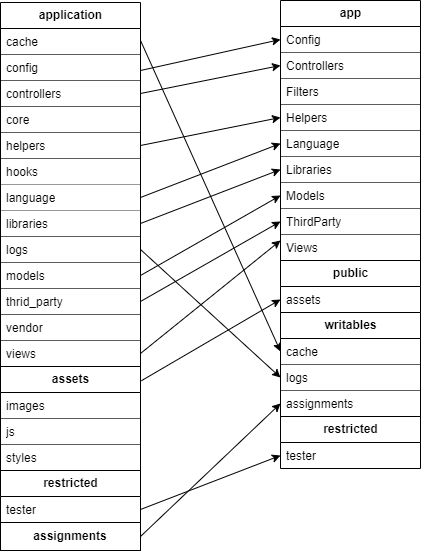
\includegraphics[scale=0.5]{dirMapping}  
	\caption[\textit{Pemindahan struktur aplikasi menuju \textit{CodeIgniter 4}}]{\textit{Pemindahan struktur aplikasi menuju \textit{CodeIgniter 4}}} 
	\label{fig:dirMapping} 
\end{figure} 

Berikut merupakan rincian direktori yang akan dipindahkan menuju \textit{CodeIgniter 4}.
\subsubsection{Application}
Direktori-direktori \texttt{application} pada \textit{CodeIgniter 3} akan dipindahkan dengan penyesuaian menuju direktori \texttt{app} terkecuali direktori \texttt{vendor}, \texttt{cache} dan \texttt{core}. Berikut merupakan direktori yang dipindahkan dari direktori \textit{application} menuju direktori \textit{app}.
\begin{itemize}
\item \verb|application/config| akan dipindahkan menuju \texttt{app/Config}.
\item \verb|application/controllers| akan dipindahkan menuju \texttt{app/Controllers}.
\item \verb|application/helpers| akan dipindahkan menuju \texttt{app/Helpers}.
\item \verb|application/languange| akan dipindahkan menuju \texttt{app/Languange}.
\item \verb|application/libraries| akan dipindahkan menuju \texttt{app/Libraries}.
\item \verb|application/models| akan dipindahkan menuju \texttt{app/Models}.
\item \verb|application/views| akan dipindahkan menuju \texttt{app/views}.
\end{itemize}

\subsubsection{\textit{Public}}
\textit{CodeIgniter 3} tidak menyediakan direktori akar berupa \textit{public} sehingga terdapat perubahan struktur dimana direktori yang sebelumnya ada pada \texttt{application} akan dipindah menuju direktori \texttt{public}. Berikut merupakan direktori yang dipindahkan menuju direktori \texttt{public}.
\begin{itemize}
\item \verb|assets| akan dipindahkan menuju \texttt{public/assets}.
\end{itemize}

Selain stuktur aplikasi diatas, \textit{SharIF Judge} memiliki dua buah direktori terpisah diluar direktori utama bernama \textit{assignments} dan \textit{tester}. Direktori \textit{assignments} ini berfungsi untuk menyimpan seluruh \textit{file} yang telah dikumpulkan sedangkan direktori \textit{tester} digunakan untuk melakukan percobaan untuk keamanan \textit{sandbox}. Kedua direktori ini harus dapat ditulis oleh \textit{PHP} sehingga akan dipindahkan menuju direktori \textit{writables}.

\subsubsection{\textit{Writables}}
Direktori ini merupakan direktori berisikan seluruh direktori yang dapat ditulis oleh \textit{PHP}. Berikut merupakan direktori yang dipindahkan menuju \textit{writables}.
\begin{itemize}
\item \verb|application/cache| akan dipindahkan menuju \texttt{writables/cache}.
\item \verb|application/log| akan dipindahkan menuju \texttt{writables/logs}.
\item \verb|assignments| akan dipindahkan menuju \texttt{writables/assignments}.
\end{itemize}

\subsection{\textit{Routing}}
\textit{Routing} pada aplikasi \textit{SharIF Judge} menggunakan \textit{auto routing} yang telah disediakan oleh \textit{CodeIgniter 3}. \textit{Auto routing} akan membentuk \textit{url} sesuai dengan \textit{controller} dan \textit{method} yang telah dibentuk tanpa harus didefinisikan secara manual. Penggunaan \textit{auto routing} seperti pada \textit{CodeIgniter 3} memiliki kekurangan pada bagian keamanan dimana \textit{filter} pada \textit{controller} dan proteksi \textit{CSRF} akan dilewati. Sehingga, konversi pada aplikasi \textit{SharIF Judge} akan menggunakan \textit{URI Routing} yang didefinisikan secara manual untuk alasan keamanan dan \textit{url} yang fleksibel. Berikut merupakan contoh \textit{route} yang didefinisikan secar a manual.
\begin{center}
\verb|$routes->post("login/register",'Login::register');|
\end{center}
\textit{Route} akan didefinisikan secara eksplisit sesuai dengan fungsi dan metodenya.

\subsection{\textit{Model, View, and Controller}}
\textit{CodeIgniter 4} memiliki perubahan baik dari kegunaan dan cara pemanggilan \textit{Model, View, and Controller}. Berikut merupakan perubahan yang terjadi:
\subsubsection{\textit{Model}}
\textit{Model} pada \textit{CodeIgniter 4} memiliki perubahan dimana \textit{model} dapat digunakan untuk mengambil data pada satu buah tabel spesifik. Konversi \textit{model} dari \textit{CodeIgniter 3} menuju \textit{CodeIgniter 4} dapat dilakukan menggunakan dua buah cara yakni:
\begin{enumerate}
\item Menggunakan \textit{Model} dari \textit{CodeIgniter 3}

\textit{Model} pada \textit{CodeIgniter 3} memiliki kekurangan dimana pengguna harus membentuk secara manual seluruh fungsi untuk mengambil, memasukan, dan memperbaharui data dari sebuah tabel spesifik pada \textit{model} tersebut. Kode \ref{kode:modelCI3} merupakan contoh fungsi yang digunakan untuk mengambil data dari sebuah tabel.
\begin{lstlisting}[caption=Contoh fungsi untuk mengambil data seluruh user, label=kode:modelCI3]
public function get_all_users()
	{
		return $this->db->order_by('role', 'asc')->order_by('id')->get('users')->result_array();
	}
\end{lstlisting}

Kode \ref{kode:modelCI3} mengambil data dari tabel \texttt{users} dengan hasil berupa \textit{array} dan diurutkan sesuai dengan \texttt{role} dan \texttt{id}nya.

\item Menggunakan \textit{Model} pada \textit{CodeIgniter 4}

\textit{CodeIgnier 4} menyediakan fungsi \textit{model} yang dapat dibentuk melalui \textit{command line} untuk sebuah tabel spesifik. Pengguna dapat membentuk \textit{model} melalui \textit{command line} menggunakan sintaks sebagai berikut.
\begin{center}
	\verb|make:model <name>|
\end{center}
\textit{Model} pada \textit{CodeIgniter 4} menyediakan fungsi untuk mengambil, memasukan, dan memperbaharui data dari sebuah tabel spesifik tanpa harus membentuk secara manual fungsi-fungsi tersebut. Pengguna dapat melakukan inisiasi dan memakai fungsi untuk mengambil data menggunakan kode berikut.
\begin{center}
	\verb|$userModel = new \App\Models\UserModel();|
\end{center}
\begin{center}
	\verb|$user = $userModel->findAll();|
\end{center}
\end{enumerate}

Kode diatas akan mengambil seluruh data dari \verb|$userModel| sesuai dengan konfigurasi yang telah dilakukan pengguna. Pengguna juga dapat melakukan \textit{create, update,} dan \textit{delete} melalui kode berikut.

\begin{lstlisting}[caption=Contoh kode untuk menghapus data pada model, label=kode:modelCI4Delete]
$this->Notifications_model->delete('notifications', array('id' => $id));

\end{lstlisting}

Konversi aplikasi \textit{SharIF Judge} akan menggunakan kedua buah cara dengan penghapusan beberapa fungsi yang terdapat pada \textit{model} dari \textit{CodeIgniter 4} seperti mengambil, menghapus, dan menambahkan data. Sedangkan untuk fungsi-fungsi lain pada \textit{SharIF Judge} akan dilakukan pembaharuan sesuai dengan dokumentasi yang telah ada.

\subsubsection{\textit{View}}
\textit{View} pada aplikasi \textit{SharIF Judge} menggunakan \textit{template engine} bernama \textit{Twig}. \textit{Twig} merupakan sebuah \textit{template engine} untuk bahasa pemrograman \textit{PHP} yang berguna untuk mempermudah dalam mebentuk tampilan sebuah aplikasi. \textit{Twig} tidak terintegrasi pada \textit{CodeIgniter 4} sehingga akan terdapat beberapa pemasangan dan perubahan pada sintaks yang telah dipasang. Selain itu, terdapat beberapa perubahan fungsi pada \textit{CodeIgniter 4} sehingga perlu dilakukan penyesuaian seperti pengubahan \textit{file extension} dari \texttt{.twig} menjadi \texttt{.php}. Konversi \textit{SharIF Judge} menuju \textit{CodeIgniter 4} akan mengubah \textit{view} yang sebelumnya menggunakan \textit{twig} menjadi menggunakan \textit{PHP} sesuai dengan dokumentasi \textit{CodeIgniter 4}. Seluruh \textit{delimiters} akan diubah menggunakan fitur yang terdapat pada \textit{CodeIgniter 4}. Kode \ref{kode:viewTwig} merupakan contoh konversi yang dilakukan.

\begin{lstlisting}[caption=Contoh \textit{view} menggunakan \textit{twig}, label=kode:viewTwig]

	<a href="{{ site_url('register') }}">Register</a> |

\end{lstlisting}

menjadi kode berikut:

\begin{lstlisting}[caption=Contoh \textit{view} menggunakan \textit{php}, label=kode:viewPHP]
<?php if($registration_enabled): ?>
	<a href="<?= site_url('register') ?>">Register</a> |
<?php endif ?>
\end{lstlisting}

Seluruh sintaks \textit{twig} akan diubah menjadi sintaks \textit{PHP} dari \textit{CodeIgniter 4} seperti yang terdapat pada kode \ref{kode:viewPHP}.

\subsubsection{\textit{Controller}}
\textit{Controller} pada \textit{CodeIgniter 4} memiliki fungsi sama dengan pada \textit{CodeIgniter 3} sehingga hanya perlu dilakukan penghapusan dan perubahan pada sintaks yang ada. Namun, terdapat perubahan pada \texttt{constructor} dimana pada \textit{CodeIgniter 4} terdapat \texttt{initController}. \textit{Constructor} pada \textit{PHP} tidak diperbolehkan untuk mengembalikan apapun sehingga terdapat beberapa pemindahan fungsi seperti \texttt{redirect()} menuju \textit{filters}. Selain itu, konversi akan tetap menggunakan \verb|__construct| dengan pemindahan beberapa sintaks menuju \texttt{initController} seperti pemanggilan \textit{helpers} dan variabel yang dapat diakses pada seluruh \textit{controller}. Berikut merupakan contoh penggunaan \texttt{initController} untuk variabel.

\begin{lstlisting}[caption=Contoh penggunaan initController untuk variabel, label=kode:initController]
protected $config;

public function initController(RequestInterface $request, ResponseInterface $response, LoggerInterface $logger)
    {
        // Do Not Edit This Line
        parent::initController($request, $response, $logger);

        // Preload any models, libraries, etc, here.

        // E.g.: $this->session = \Config\Services::session();
        $this->config = Config('Secrets');
    }
\end{lstlisting}

Kode \ref{kode:initController} akan memanggil variabel \verb|$config| berisikan data dari \textit{file config} \texttt{Secrets.php} yang dapat digunakan seluruh \textit{controller}.

Fungsi lainnya akan dipindahkan sesuai dengan yang ada pada \textit{CodeIgniter 3} dengan pembaharuan sesuai dengan dokumentasi \textit{CodeIgniter 4}. Selain pembaharuan, akan terdapat pemindahan variabel \textit{global} yang sebelumnya telah diinisiasikan menuju \textit{controller}.

\subsection{\textit{Libraries}}
\textit{Libraries} pada \textit{CodeIgniter 3} memiliki perubahan dan penghapusan pada \textit{CodeIgnier 4} sehingga perlu dilakukan pembaharuan. Berikut merupakan \textit{libraries} yang dipakai pada \textit{SharIF Judge}:

\subsubsection{\textit{Emails}}
\textit{Emails} pada \textit{CodeIgnier 4} terdapat perubahan sintaks dan cara pemanggilan sehingga akan dipindahkan sesuai dengan sintaks yang baru. Sintaks berubah dari yang sebelumnya menggunakan \textit{snakecase} menjadi menggunakan \textit{camelcase}. Kode \ref{kode:emailslibbab3} merupakan contoh penggunaan \textit{library email}.

\begin{lstlisting}[caption=Contoh perubahan \textit{library emails}, label=kode:emailslibbab3]
$this->email->setFrom($this->settings_model->get_setting('mail_from'), $this->settings_model->get_setting('mail_from_name'));
				$this->email->setTo($user[1]);
				$this->email->setSubject('SharIF Judge Username and Password');
				$text = $this->settings_model->get_setting('add_user_mail');
				$text = str_replace('{SITE_URL}', base_url(), $text);
				$text = str_replace('{ROLE}', $user[4], $text);
				$text = str_replace('{USERNAME}', $user[0], $text);
				$text = str_replace('{PASSWORD}', htmlspecialchars($user[3]), $text);
				$text = str_replace('{LOGIN_URL}', base_url(), $text);
				$this->email->setMessage($text);
				$this->email->send()
\end{lstlisting}

Kode \ref{kode:emailslibbab3} memiliki sintaks dengan nama sama namun terdapat perubahan menjadi \textit{camelcase}.

\subsubsection{\textit{Working with Uploaded Files}}
\textit{Upload} akan digantikan dengan fungsi \textit{Working with oploaded files} dengan beberapa penggantian dan penghapusan fungsi. \textit{Working with uploaded files} terdapat perubahan pada beberapa sintaks dan validasi terhadap \textit{file} yang telah diunggah. Kode \ref{kode:uploadconvbab3} merupakan perubahan yang terdapat dalam melakukan \textit{upload} sebuah file.

\begin{lstlisting}[caption=Contoh perubahan \textit{library upload}, label=kode:uploadconvbab3]
$zip_uploaded = $this->request->getFile('tests_desc');
$pdf_uploaded->move("$assignment_dir");
\end{lstlisting}

Kode \ref{kode:uploadconvbab3} merupakan perubahan dalam melakukan \textit{upload} sebuah file. Sintaks \texttt{getFile} akan mengambil file bernama \texttt{tests\_desc} yang dikirimkan oleh pengguna. Sintak selanjutnya akan memindahkan file tersebut menuju direktori yang terlah dibentuk.

\subsubsection{Request}
\textit{Input} akan digantikan menggunakan fungsi \textit{request} dengan perubahan beberapa fungsi. Kode \ref{kode:requestconvbab3} merupakan perubahan yang terdapat dalam menerima \textit{input} dari pengguna.

\begin{lstlisting}[caption=Contoh perubahan \textit{library request}, label=kode:requestconvbab3]
$this->request = \Config\Services::request(); 
$names => $this->request->getPost('name'),
\end{lstlisting}

Kode \ref{kode:requestconvbab3} merupakan perubahan dalam menerima data yang dikirim melalui \textit{post}.Sintaks pertama akan melakukan inisiasi terhadap \textit{library} tersebut namun inisiasi tersebut hanya diperlukan pada \textit{model} karena fungsi ini sudah terdapat pada \textit{controller}.Sintaks baris kedua akan mengambil data bernama \textit{name} yang telah dikirimkan oleh pengguna melalui \textit{post}. Konversi aplikasi \textit{SharIF Judge} akan menggunakan fungsi ini dengan beberapa perubahan sintaks sesuai dengan dokumentasinya.

\subsubsection{\textit{Validation}}
\textit{Form\_validation} akan digantikan menggunakan fungsi \textit{validation} dengan perubahan dan pengapusan beberapa fungsi. Berikut merupakan contoh pembentukan aturan untuk mengumpulkan sebuah data pada \textit{form}.
\begin{center}
\verb|$validate->setRule('username', 'username', 'required|min\_length[3]|max\_length[20]);|
\end{center}
Sintaks diatas akan melakukan validasi terhadap \textit{input} yang akan masukan oleh pengguna. Namun, \textit{CodeIgniter 4} tidak menyediakan fungsi \texttt{form\_error} sehingga akan diubah dengan menggunakan fungsi baru bernama \texttt{validation\_errors()}. Fungsi tersebut dapat digunakan untuk mengembalikan \textit{error} apabila terdapat data yang tidak sesuai dengan aturan. \textit{Error} tersebut dapat ditampilkan pada halaman \textit{view} menggunakan sintaks berikut.

\begin{center}
\verb|<?= $validation->getError('username'); ?>|
\end{center}

Sintaks diatas akan mengembalikan \textit{error} terhadap \textit{form} dengan nama \textit{username} apabila tidak sesuai dengan aturan yang sudah ditentukan. Variabel \texttt{validation} akan dikirimkan dari \textit{controller} berisikan \textit{library} dari \textit{validation} tersebut.

\subsubsection{\textit{Zip Archive}}
\label{subsubsec:ziparchivebab3}
\textit{Zip Encoding} dan \textit{Unzip} akan digantikan dengan fungsi PHP \textit{zip archive} karena sudah tidak tersedia pada \textit{CodeIgniter 4}. Fungsi \textit{zip archive} terdapat beberapa perbedaan sehingga akan disesuaikan dengan fungsi-fungsi yang ada.
\\
\textit{Library} yang terdapat pada \textit{CodeIgniter 4} juga dapat di\textit{extend} dan dibentuk sesuai dengan kebutuhan. Berikut merupakan \textit{library} yang dibentuk oleh pengguna.

\begin{lstlisting}[caption=Contoh perubahan penggunaan\textit{library ZipArhive} untuk melakukan \textit{zip}, label=kode:ziparchivebab3]
		$this->zip = new \ZipArchive();
		$this->zip->open($zipname, ZipArchive::CREATE);
		$this->zip->addFile($file_path,"{$item['username']}/p{$item['problem']}.".filetype_to_extension($item['file_type']));
\end{lstlisting}

Kode \ref{kode:ziparchivebab3} merupakan perubahan dalam melakukan \textit{zip} sebuah file. Baris pertama akan melakukan inisiasi terhadap \textit{ZipArchive} sedangkan baris kedua akan membuka file \textit{zip}. Terakhir baris terakhir akan memasukan file bernama \textit{file\_path} menuju zip yang terdapat pada \textit{array item}. Selain untuk membentuk file \textit{zip}, \textit{zip arhive} juga dapat melakukan \textit{unzip} terhadap file. Kode \ref{kode:ziparchiveunzipbab3} merupakan penggunaan \textit{ZipArchive} dalam melakukan \textit{unzip}.
\begin{lstlisting}[caption=Contoh perubahan penggunaan\textit{library ZipArhive} untuk melakukan \textit{unzip}, label=kode:ziparchiveunzipbab3]
		$this->unzip = new ZipArchive();
			// Create a temp directory
			$tmp_dir = "$assignments_root/$tmp_dir_name";
			// Extract new test cases and descriptions in temp directory
			$this->unzip->open("$assignments_root/".$zip_uploaded->getName());
			$extract_result = $this->unzip->extractTo($tmp_dir);
\end{lstlisting}

Kode \ref{kode:ziparchiveunzipbab3} merupakan perubahan dalam melakukan \textit{unzip} dalam \textit{ZipArchive}. Baris pertama akan melakukan inisiasi terhadap \textit{ZipArchive} sedangkan baris kedua membentuk sebuah direktori sementara bernama \textit{assignments\_root/shj\_tmp\_directory}. Baris ketiga akan membuka sebuah \textit{zip} pada \textit{assignments\_root} dengan nama yang dibentuk. Baris terakhir akan melakukan \textit{extract} file pada direktori yang sudah dibentuk.

\subsubsection{\textit{Twig}}
\textit{Library} ini tidak akan digunakan untuk membentuk \textit{view} pada \textit{CodeIgniter 4} namun, akan ada penggunaan sebuah fungsi \textit{Twig} yang akan dibentuk pada direktori \texttt{app/Libraries}. Fungsi tersebut bernama \texttt{extra\_time\_formatter} yang memiliki fungsi untuk mengubah input yang diberikan menjadi format jam dikali enam puluh menit. 

\subsubsection{\textit{Unzip}}
\textit{Library} ini tidak akan digunakan dan digantikan oleh \textit{ZipArchive} yang disediakan oleh PHP. Terdapat perubahan sintaks pada \textit{ZipArchive} sehingga akan disesuaikan. Perubahan dapat dilihat pada subbab \ref{subsubsec:ziparchivebab3} kode \ref{kode:ziparchiveunzipbab3}.

\subsubsection{\textit{Password\_hash}}
\textit{Library} ini tidak akan digunakan dan akan digantikan oleh \textit{password hash} yang disediakan oleh PHP .\textit{Library} \textit{Password\_hash} merekomendasikan pegguna untuk menggunakan fungsi \textit{native} yang disediakan oleh PHP apabila aplikasi mendukung PHP versi 5.5 ke atas. Sehingga, akan dilakukan konversi menggunakan fungsi yang disediakan oleh PHP bernama \texttt{password\_hash()}. Seluruh penggunaan \textit{library} ini akan diubah menggunakan fungsi yang disediakan oleh PHP dengan metode \textit{hashing} sama yaitu \textit{CRYPT\_BLOWFISH}. Perubahan fungsi \textit{hashing} ini bersifat \textit{backward compatible} sehingga dapat menggunakan \textit{database} aplikasi terdahulu tanpa perlu membentuk data baru. Berikut merupakan contoh pengubahan kode dari \textit{phpass} menjadi \textit{password\_hash}.

\begin{center}
\verb|'password' => $this->password_hash->HashPassword($password)|
\end{center}
menjadi
\begin{center}
\verb|'password' => password_hash($password,PASSWORD_BCRYPT)|
\end{center}

Sintaks \texttt{password\_hash()} diatas menerima dua buah parameter yakni data yang ingin di enkripsi dan tipe enkripsi. Enkripsi akan menggunakan sintaks \texttt{PASSWORD\_BCRYPT} yang menggunakan tipe \textit{hash} berupa \texttt{CRYPT\_BLOWFISH}.

\subsubsection{\textit{MY\_Form\_validation}}
\textit{Library MY\_Form\_validation} akan dipindahkan menuju direktori \texttt{app/Libraries}. \textit{Library} ini akan digunakan kembali dengan perubahan \textit{extends} menjadi menuju \texttt{Validation}, penghapusan sintaks \texttt{defined} , dan akan ada penambahan \textit{namespace} pada baris awal file. Kode \ref{kode:myformvalidationbab3} merupakan contoh penambahan \textit{namespace} dan penggantian \textit{extends} pada \textit{library} ini.
\begin{lstlisting}[caption=Contoh perubahan \textit{library MY\_Form\_validation} pada \textit{CodeIgniter 4}, label=kode:myformvalidationbab3]
namespace App\Libraries;

use CodeIgniter\Validation\Validation;

class MY_Form_validation extends Validation
\end{lstlisting}
Kode \ref{kode:myformvalidationbab3} mengapus sintaks \texttt{defined} dan menggantikannya dengan penambahan \textit{namespace}. Selain itu, kelas \textit{library} akan \textit{extends} \textit{Validation}.

\subsubsection{\textit{Parsedown}}
\textit{Library Parsedown} akan dipindahkan menuju direktori \texttt{app/Libraries}. \textit{Library} ini akan digunakan kembali dengan penambahan \textit{namespace} pada baris awal file dan penghapusan sintaks \texttt{defined}.  Kode \ref{kode:parsedownbab3} merupakan contoh penambahan \textit{namespace} dan juga penambahan sintaks \textit{defined}.
\begin{lstlisting}[caption=Contoh perubahan \textit{library Parsedown} pada \textit{CodeIgniter 4}, label=kode:parsedownbab3]
namespace App\Libraries;

class Parsedown
\end{lstlisting}
Kode \ref{kode:parsedownbab3} menghapus sintaks \texttt{defined} dan menggantikannya dengan penambahan \textit{namespace}.
\subsubsection{\textit{Phpexcel}}
\textit{Library} ini akan digunakan kembali namun tidak akan dipindahkan menuju \texttt{app/Libraries}. \textit{Library} akan dilakukan instalasi melalui \textit{composer} dengan sintaks berikut:
\begin{center}
	\verb|composer require phpoffice/phpexcel|
\end{center}
Sintaks diatas akan dijalankan pada akar dari aplikasi dan tidak terdapat perubahan terhadap penggunaan sintaks ini.
\subsubsection{\textit{Shj\_pagination}}
\textit{Library} ini akan digunakan kembali dan dipindahkan menuju direktori \texttt{app/Libraries}. Selain itu, terdapat penambahan \textit{namespace} pada baris awal file dan penghapusan sintaks \textit{defined}.

\subsection{\textit{Configuration}}
\textit{Configuration} terdapat perubahan nama dari yang sebelumnya \texttt{application/config/config.php} menjadi \texttt{app/Config/App.php} dan penambahan \textit{file} dengan nama \texttt{app/Config/Secrets.php}. Berhubung dengan perubahan nama tersebut, terdapat beberapa perpindahan sintaks menuju direktori baru tersebut. Berikut merupakan sintaks yang dipindahkan menuju \texttt{app/Config/Security.php}:
\begin{itemize}
\item \verb|$config['csrf_protection'] = TRUE;|
\item \verb|$config['csrf_token_name'] = 'shj_csrf_token';|
\item \verb|$config['csrf_cookie_name'] = 'shjcsrftoken';|
\item \verb|$config['csrf_expire'] = 7200;|
\item \verb|$config['csrf_regenerate'] = FALSE;|
\end{itemize}

\textit{Configurations} yang telah dipindahkan akan diubah dari yang sebelumnya menggunakan \textit{array} menjadi menggunakan \textit{variable}. Seluruh \textit{configurations} pada \textit{CodeIgniter 3} akan dipindahkan menuju \textit{CodeIgniter 4} sesuai dengan direktorinya dan fungsinya. Sedangkan \texttt{app/Config/App.php} dan dipindahkan menuju file \texttt{.env} karena alasan kemudahan untuk penggantian \textit{environment} dalam melakukan \textit{deploy}.

\subsection{\textit{Database}}
\textit{Database} pada \textit{CodeIgniter 4} fungsi yang sama pada \textit{CodeIgniter 3} sehingga akan dilakukan pemindahan konfigurasi sesuai dengan yang ada pada \textit{CodeIgniter 3}. Namun, terjadi beberapa perubahan pada sintaks untuk melakukan koneksi ke \textit{database} dan beberapa sintaks untuk melakukan \textit{query}. Sintaks koneksi \textit{database} akan berubah dari \texttt{\$this->load->database();} menjadi \texttt{db = db\_connect()}. Selain itu, pemanggilan fungsi \textit{query builder} berubah menggunakan \textit{camelcase} dari yang sebelumnya menggunakan \textit{snakecase}. Seperti dari yang sebelumnya menggunakan sintaks \texttt{get\_where} menjadi \texttt{getWhere}.

\textit{Database} pada aplikasi \textit{SharIF Judge} menggunakan \textit{autoload} yang dapat memuat beberapa fungsi secara otomatis. Berikut merupakan contoh penggunakan \textit{autoload} pada \textit{CodeIgniter 3}.
\begin{center}
\verb|$autoload['libraries'] = array('database');|
\end{center}
Sintaks diatas memuat \textit{library database} dan akan  ditambahkan pada \textit{file} \texttt{autoload.php}. Namun, pada konversi ini tidak akan menggunakan \textit{autoload} karena \textit{CodeIgniter 3} tidak mengikuti standar \textit{PSR 4} sehingga pada \textit{CodeIgniter 4} akan dimuat menggunakan \texttt{db = db\_connect()} pada \texttt{initController}.

\subsection{\textit{Helpers}}
\textit{Helpers} tidak terdapat banyak perubahan namun, terdapat perubahan pemanggilan \textit{helpers} dan beberapa penghapusan \textit{helpers}. Berikut merupakan \textit{helpers} yang dihapus dan diubah cara pemanggilannya.
\begin{itemize}
\item \textit{Download Helper}
\textit{Helper} ini sudah tidak tersedia pada \textit{CodeIgniter 4} sehingga perlu dilakukan pengubahan dengan menggunakan fungsi \textit{HTTP Response}. \textit{HTTP Response} menyediakan fungsi bernama \textit{Force File Download} yang berguna untuk mengunduh sebuah \textit{file} menuju perangkat pengguna. Fungsi ini dapat dipanggil menggunakan sintaks berikut.

\begin{center}
 \verb|return $this->response->download($name, $data);|
\end{center}

Sintaks diatas mengembalikan \textit{file} yang ingin diunduh pengguna dengan dua buah parameter. Parameter pertama berupa nama \textit{file} yang ingin diunduh sedangkan parameter kedua merupakan data dalam \textit{file} tersebut.

\item \texttt{redirect()} \\
Fungsi ini memiliki perubahan pada \textit{CodeIgniter 4} dimana \texttt{redirect()} tidak langsung mengarahkan kepada \textit{url} yang dibentuk. Pengguna harus mengembalikan fungsi \textit{redirect()} menggunakan \texttt{return} dengan sintaks sebagai berikut.
\begin{center}
 \verb|return redirect()->to('login/form')|
\end{center} 

Sintaks diatas akan mengembalikan pengguna menuju \textit{url} \texttt{login/form} yang sudah dibentuk pada \textit{routes}.

\end{itemize}

Konversi \textit{helpers} akan dipindahkan dari yang sebelumnya menggunakan \textit{autoload} menuju \texttt{initController} dengan menambahkan pada variabel \textit{helpers}.
